\documentclass{article}
\usepackage{fullpage}
\usepackage{overture}
\usepackage{hyphenat}
\usepackage[pdftex]{hyperref}

\hypersetup{
    colorlinks,%
    citecolor=black,%
    filecolor=black,%
    linkcolor=red,%
    urlcolor=blue
}

\usepackage{amsmath}

\usepackage[utf8]{inputenc}
\usepackage[T1]{fontenc}
\usepackage[portuguese]{babel}
\usepackage{longtable}
\usepackage{pifont}

\usepackage{float}
\usepackage{listings}
\usepackage{makeidx}  % allows for indexgeneration
\usepackage[center]{caption}
\usepackage{url}
\usepackage{graphicx}
\usepackage{fancyvrb}
\usepackage{pdfpages}
\usepackage{tabularx}
\usepackage{array}


% Um comando simples para escrever os emails com links do tipo mailto:
\newcommand{\email}[1]{\href{mailto:#1}{\texttt{#1}}}

% Uma forma mais simples de colocar vistos na matriz de rastreabilidade
\newcommand{\checkmark}[0]{\ding{51}}


\title{\emph{Mastermind}}

\author{João Alves - \email{ei08083@fe.up.pt} \\
  Rolando Pereira - \email{ei08150@fe.up.pt}}




\begin{document}

%\maketitle

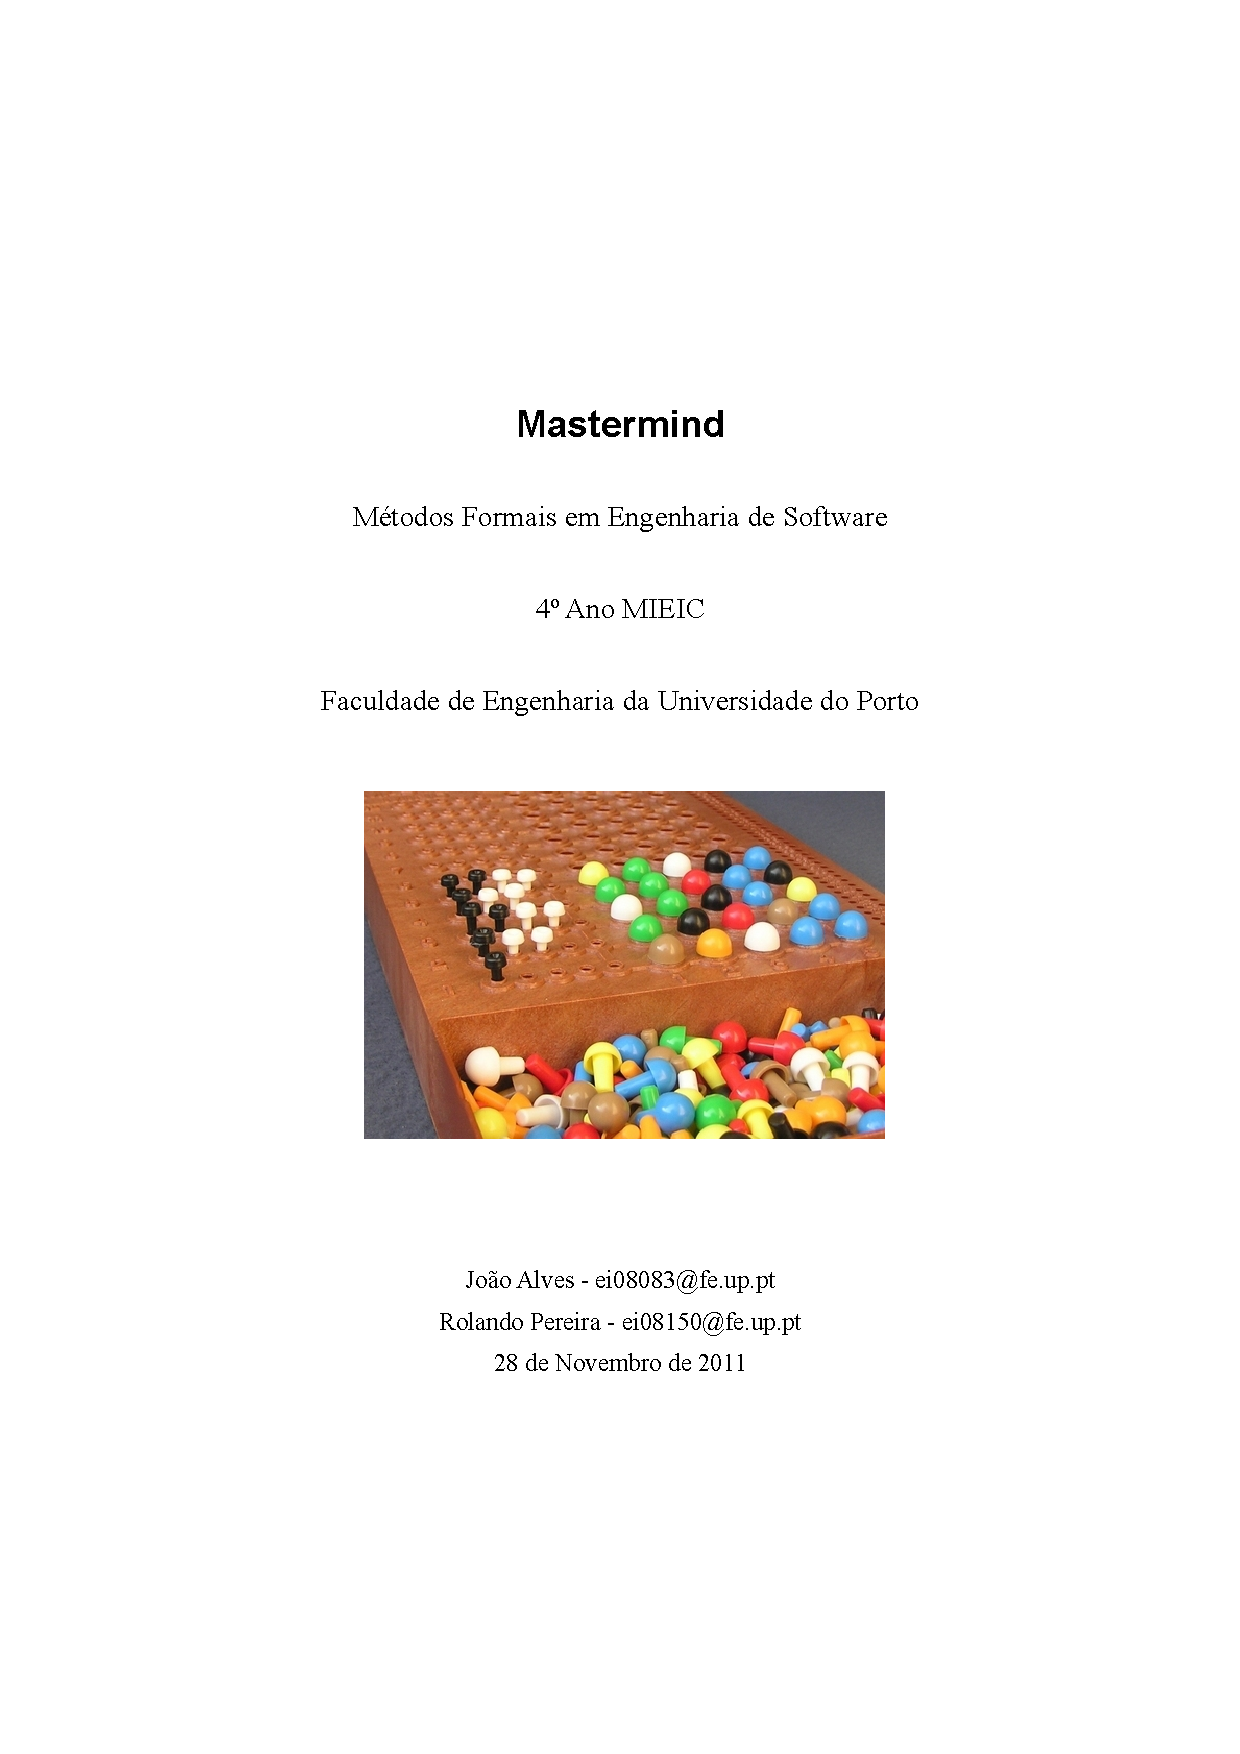
\includepdf{capa.pdf}


\tableofcontents

\newpage


\section{Introdução}
Este relatório foi realizado no âmbito da unidade curricular de
Métodos Formais Formais em Engenharia de Software do 4º ano do
Mestrado Integrado em Engenharia Informática e Computação da Faculdade
de Engenharia da Universidade do Porto.

Este documento especifica, utilizando a linguagem VDM++, um modelo
formal das regras do conhecido jogo Mastermind, pretendendo assim
dotar os elementos do grupo de capacidades que lhes permitam criar no
futuro modelos formais que permitam representar e interagir com outros
sistemas.

Este relatório terá a seguinte estrutura: primeiro iremos descrever as
regras do jogo Mastermind, sendo depois enumerados os requisitos e
restrições que foram implementados neste modelo.

Após essa descrição será demonstrado como é que as restrições foram
implementadas no modelo escrito em VDM++.

De seguida iremos explicar o método usado para escrever e ler objetos
a partir do disco, e quais as razões pelas quais esta funcionalidade
não está implementada no código Java gerado.

Iremos depois descrever a bateria de testes utilizada para testar o
modelo, e será mostrada tanto a matriz de rastreabilidade como o
diagrama de classes gerado pelo Enterprise Architect.

Será depois colocado o código completo das classes utilizadas neste
trabalho bem como a sua cobertura por parte dos testes definidos
anteriormente.

Por fim será descrito a funcionalidade de análise de consistência do
modelo disponível nas ferramentas utilizadas para desenvolver este
modelo.

Na realização deste trabalho foram gastas aproximadamente 60 horas para especificar o
modelo, 2 horas para construir e executar os casos de teste e 10 horas
para gerar o código adicional necessário para fornecer uma
implementação a funcionar

\section{Descrição das regras do Mastermind}

O Mastermind é um jogo de tabuleiro jogado entre 2 jogadores, em que
um deles cria um código secreto e o outro tenta-o descobrir num
determinado número de tentativas. Um exemplo de um tabuleiro, neste
caso num jogo de computador, pode ser visto na figura
\ref{fig:tabuleiro_mastermind}.

\begin{figure}[h!]
  \centering
    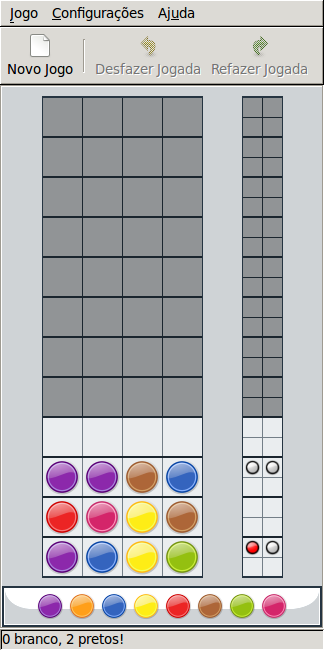
\includegraphics[scale=0.30]{gnome-mastermind.png}    
  \caption{Software que permite jogar o jogo Mastermind. Na situação
    mostrada o \emph{codebreaker} já efetuou 3 tentativas para adivinhar o código.}
  \label{fig:tabuleiro_mastermind}
\end{figure}



Inicialmente, o tabuleiro onde se vai efetuar o jogo encontra-se
limpo. Nesta altura, um dos jogadores, designado por \emph{codemaker}, cria,
utilizando as 6 cores disponíveis, um código de 4 cores. Este código
pode conter cores repetidas. Por exemplo, Azul, Azul, Azul, Azul é um
código válido.

Este código fica escondido, através de uma proteção existente no
tabuleiro, do outro jogador, designado por \emph{codebreaker}.

Após a criação do código por parte do \emph{codemaker}, o \emph{codebreaker} têm 12
tentativas para o tentar descobrir.

Cada tentativa processa-se da seguinte forma:
%
\begin{enumerate}
\item O \emph{codebreaker} escolhe um combinação de 4 cores que pensa ser a
  que o \emph{codemaker} criou;
\item O \emph{codemaker} observa a combinação escolhida pelo \emph{codebreaker} e
  compara-a com a que escolheu antes de começar o jogo;
\item Por cada cor que seja igual e esteja no mesmo sítio que uma cor
  do código original, o \emph{codemaker} coloca uma peça preta ao lado do
  código criado pelo \emph{codemaker};
\item Por cada cor que seja igual, mas esteja num sítio diferente que
  uma cor do código original, o \emph{codemaker} coloca uma peça branca ao
  lado do código criado pelo \emph{codemaker};
\end{enumerate}

Isto repete-se até que uma das seguintes situações ocorra:
%
\begin{enumerate}
\item O \emph{codemaker} coloca 4 peças pretas ao lado de uma tentativa feita
  pelo \emph{codebreaker}, indicando a este que o seu código está correto;
\item O \emph{codebreaker} não consegue descobrir o código criado pelo
  \emph{codemaker} no número de tentativas disponíveis.
\end{enumerate}

Se alguma destas situações ocorrer, então aquele jogo termina.

São atribuídos pontos ao \emph{codemaker} da seguinte forma:
%
\begin{itemize}
\item Se o \emph{codebreaker} descobriu o código, então o \emph{codemaker} ganha um
  número de pontos igual ao número de tentativas feitas pelo \emph{codebreaker};
\item Se o \emph{codebreaker} não descobriu o código, então o \emph{codemaker} ganha
  um número de pontos igual ao número de tentativas feitas mais 1.
\end{itemize}

Após este jogo terminar é realizado um outro jogo em que os papéis dos
jogadores estão invertidos, ou seja, o jogador que fez de \emph{codemaker}
passa a ser o \emph{codebreaker} e assim sucessivamente.

É então jogado um novo jogo como foi descrito anteriormente.

No final desse jogo, a partida termina e ganha quem tiver tido o maior
número de pontos, ou seja, ganha quem tiver feito o código mais
difícil de descobrir.



\section{Lista de Requisitos do Sistema de Software}
\label{sec:lista_requisitos}

Inicialmente, foi-nos indicado no enunciado deste projeto que o
sistema deveria cumprir com estes 3 requisitos:

\begin{enumerate}
\item Perguntar ao sistema qual o número de peças com a cor certa e no
  sítio certo e qual o número de peças com a cor certa mas no sítio
  errado de cada tentativa;
\item Calcular o número de tentativas que o \\emph{codebreaker} precisou para
  adivinhar o código;
\item Guardar a informação sobre um campeonato com várias equipas e
  calcular a soma do número de tentativas que a equipa vencedora precisou
\end{enumerate}

A partir desses três requisitos pedidos e da descrição das regras do
Mastermind efetuada anteriormente, criámos um conjunto de requisitos
que o sistema tinha que implementar para funcionar corretamente:

\begin{enumerate}
\item Num jogo, com duas equipas, existem sempre duas partidas, em que
  cada equipa tenta quebrar o código definido pela adversária;
\item Dado um jogo, com duas equipas, deve ser possível a cada equipa
  definir o código a ser quebrado pela equipa adversária;
\item Em cada partida, cada equipa deve poder realizar uma tentativa
  de encontrar a solução do tabuleiro;
\item Dada uma tentativa, num determinado tabuleiro, deve ser possível
  saber quantas peças estão com a cor certa no lugar certo;
\item Dada uma tentativa, num determinado tabuleiro, deve ser possível
  saber quantas peças estão com a cor certa no lugar errado;
\item Após uma tentativa, deve ser possível verificar se a solução foi
  encontrada;
\item Deve ser possível calcular o número de tentativas que foram
  necessárias para adivinhar a solução;
\item Deve ser possível criar um campeonato, onde participem várias
  equipas;
\item Deve ser possível adicionar equipas ao campeonato;
\item As equipas que participam num determinado jogo de um determinado
  campeonato, têm que estar inscritas no campeonato;
\item Dada uma equipa, deve ser possível obter a sua pontuação num
  dado campeonato. Esse valor depende do número de tentativas que as
  equipas adversárias gastaram para adivinhar a solução;
\item Um campeonato tem que ter no minimo 2 equipas;
\item Deve ser possível gravar um campeonato para um ficheiro e
  restaurá-lo mais tarde;
\item Deve ser possível adicionar jogos aos campeonatos.
\end{enumerate}

\subsection{Restrições necessárias para o funcionamento correto do sistema}

Foram também identificadas um conjunto de restrições que o sistema
tinha que cumprir para funcionar corretamente:

\begin{enumerate}
\item Após a solução de um tabuleiro ter sido encontrada, não é possível fazer mais
  nenhuma jogada nele;
\item Só é possível efetuar uma tentativa se o jogo ainda não tiver terminado;
\item As cores usadas nos códigos têm que pertencer a um conjunto de 6
  cores definidos previamente;
\item Cada tabuleiro só aceita tentativas e soluções com 4 elementos;
\item O número máximo de tentativas de cada tabuleiro é 8, 10, ou 12;
\item O número de peças com a cor certa no sítio certo não pode ser
  superior ao tamanho da solução do tabuleiro;
\item O número de peças com a cor certa, mas no sítio errado não pode
  ser superior ao tamanho da solução do tabuleiro;
\item O número de equipas num campeonato tem de ser um número par
  maior ou igual a 2;
\item As equipas que participam nos jogos de um campeonato têm que
  estar inscritas nesse campeonato;
\end{enumerate}


\section{Especificação, em VDM++, das restrições identificadas.}

Tendo enumerado agora as restrições que o sistema deve cumprir para
funcionar corretamente, iremos agora explicar como estas foram
implementadas no modelo de VDM.

A primeira restrição, que indica que a após a solução de um tabuleiro
ter sido encontrada não é possível fazer mais nenhuma jogada nele foi
implementada através da pré-condição implementada no operador
``makeAPlay'' da classe Board.

\begin{vdm_al}
  public makeAPlay : seq1 of Color`Color ==> ()
  makeAPlay (attempt) == ...
  pre len attempt = attemptLength and
      not isGameOver()
  post attempts = attempts~ ^ [attempt];
\end{vdm_al}

Como se pode ver pela pós-condição do operador ``isGameOver'' se a
solução já tiver sido encontrada, então este operador irá
garantidamente devolver ``true'' o que fazer com que a pré-condição do
operador ``makeAPlay'' seja falsa.

\begin{vdm_al}
  public isGameOver : () ==> bool
    isGameOver () == ...
  post RESULT = (isSolutionCracked() or len attempts = maxAttempts);
\end{vdm_al}

O operador ``isSolutionCracked'' verifica simplesmente se a solução
está na sequência de tentativas realizadas.

\begin{vdm_al}
  -- Return true if the correct code has been found
  public isSolutionCracked : () ==> bool
    isSolutionCracked () == return solution in set elems attempts
  post solution in set elems attempts => RESULT = true;
\end{vdm_al}

Como foi mostrado anteriormente, a definição de ``isGameOver'' devolve
o valor ``true'' quando o tamanho da sequência de tentativas for igual
ao número máximo de tentativas definidas para aquele tabuleiro (valor
dado pela variável ``maxAttempts''). Assim, a restrição 2 ``Só é
possível efetuar uma tentativa se o jogo ainda não tiver terminado'' é
também implementada com o uso a uma pré-condição no operador
``makeAPlay''.

Para implementar a restrição 3, que indica que uma cor usada num
tabuleiro tem que pertencer a um conjunto de cores previamente
definido foi criada uma invariante sobre o tipo Color definido na
class Color, que indica que cada variável do tipo Color têm que ser
uma das seguintes cores: ``b''lue, ``g''reen, ``r''ed, ``o''range,
``y''ellow, ``m''agenta.

\begin{vdm_al}
  types
    public Color = char
    inv color == color in set {'b', 'g', 'r', 'o', 'y', 'm'};
\end{vdm_al}

Para implementar a restrição 4, que limita o tamanho das soluções e
tentativas feitas num tabuleiro a sequências de 4 cores foram escritas
um conjunto de pré-condições em diversos operadores das classes
``Board'', ``Championship'' e ``Game''.

Primeiro, para facilitar a compreensão do código, foi criada a
seguinte constante na classe ``Board'':

\begin{vdm_al}
  values
  public attemptLength : nat1 = 4;
\end{vdm_al}

E foi também definida esta invariante sobre a variável ``attempts''
que impede que ela contenha sequências com um tamanho diferente do
valor que está em ``attemptLength'':

\begin{vdm_al}
  inv forall attempt in set elems attempts & len attempt = attemptLength and
    len attempts <= maxAttempts;
\end{vdm_al}

O mesmo foi feito para a variável ``solution'' que contêm o código a
quebrar do tabuleiro:

\begin{vdm_al}
  inv len solution = attemptLength;
\end{vdm_al}

Apesar de estas invariantes serem suficientes para cumprir com a
restrição indicada, a fim de se conseguir detetar este tipo de erros o
mais cedo possível, foram também criadas as seguintes pré-condições
nos construtores da classe ``Board'':

\begin{vdm_al}
  public Board : seq1 of Color`Color ==> Board
  Board (correctPlay) == ...
  pre len correctPlay = attemptLength
  post solution = correctPlay and
    attempts = [];
\end{vdm_al}

\begin{vdm_al}
  public Board : seq1 of Color`Color * nat1 ==> Board
  Board (correctPlay, maxNumberOfTries) == ...
  pre len correctPlay = attemptLength and
    maxNumberOfTries in set maxAttemptsAvailable
  post solution = correctPlay and
    maxAttempts in set maxAttemptsAvailable;
\end{vdm_al}

No caso do construtor ``Board()'' como este não recebe nenhuma solução
do utilizador esta é gerada aleatoriamente pelo computador então a
restrição foi colocada na pós-condição em vez de se meter na
pré-condição:

\begin{vdm_al}
  public Board : () ==> Board
  Board() == ...
  post len solution = attemptLength and attempts = [];
\end{vdm_al}

Esta restrição foi também colocada como pré-condição do operador
``makeAPlay'' da classe ``Board'', devido ao fato de a tentativa que
vai ser inserida no tabuleiro também precisar de ter um comprimento
igual a ``attemptLength''.

\begin{vdm_al}
  public makeAPlay : seq1 of Color`Color ==> ()
    makeAPlay (attempt) == ...
  pre len attempt = attemptLength and
    not isGameOver()
  post attempts = attempts~ ^ [attempt];
\end{vdm_al}

Foi também implementada esta restrição no operador ``addGame'' da
classe ``Championship'' de forma a impedir que o sistema crie jogos
cujas soluções tenham um comprimento diferente a ``attemptLength''.

\begin{vdm_al}
  public addGame : map String to (seq of Color`Color) ==> Game
  addGame(teamsSolutions) == ...
  pre dom teamsSolutions subset teams and
    dom teamsSolutions not in set oldMatchups() and
    forall solution in set rng teamsSolutions & len solution = Board`attemptLength
  post RESULT in set games;
\end{vdm_al}

E por fim, esta restrição foi implementada como uma pré-condição no construtor
``Game(teamsSolutions, championship)'' pois este construtor é
responsável por criar objetos da classe ``Board'' e assim impedimos o
sistema de tentar criar jogos que tivessem solução que quebrassem esta
restrição.

\begin{vdm_al}
  public Game : map String to seq1 of Color`Color * Championship ==> Game
  Game (teamsSolutions, championship) == ...
  pre card (dom teamsSolutions) = 2 and
    forall team in set dom teamsSolutions &
      team in set championship.getTeams() and
    forall solution in set rng teamsSolutions &
      len solution = Board`attemptLength

  post forall team in set (dom gameInstances) &
    let opponentTeam = dom teamsSolutions \ {team} in
      {gameInstances(team).getSolution()} =
      rng (opponentTeam <: teamsSolutions);
\end{vdm_al}


Para implementar a restrição 5, que indica que o número máximo de
tentativas que o \emph{codebreaker} pode efetuar têm que ser igual a 8, 10 ou
12, foi criado um conjunto na classe ``Board'' que guarda esses
valores.

\begin{vdm_al}
  public maxAttemptsAvailable : set of nat1 = {8, 10, 12};
\end{vdm_al}

Para guardar de fato o valor do número máximo de tentativas de cada
instância da classe ``Board'' foi criada uma variável ``maxAttempts''
que guarda esse valor. Esta variável tem por defeito o valor 12.

\begin{vdm_al}
  private maxAttempts : nat1 := 12;
\end{vdm_al}

Foi também definida uma invariante sobre essa variável que indica que
o valor dela têm que pertencer aos valores máximos permitidos pelas
regras do jogo.

\begin{vdm_al}
  inv maxAttempts in set maxAttemptsAvailable;
\end{vdm_al}

Tal como já foi anteriormente mostrado, a variável ``attempts'' também
contêm uma invariante que impede que o comprimento dela seja maior que
o valor de ``maxAttempts''.

\begin{vdm_al}
  inv forall attempt in set elems attempts & len attempt = attemptLength and
    len attempts <= maxAttempts;
\end{vdm_al}

Mais uma vez, apesar de estas duas invariantes serem suficientes para
garantir a restrição do tamanho do tabuleiro ser 8, 10 ou 12, foi
também adicionado código às pré-condições do construtor
``Board(correctPlay, maxNumberOfTries)'' e do operador ``makeAPlay''.

Esta restrição foi então colocada na pré-condição do construtor
``Board(correctPlay, maxNumberOfTries)'', forçando assim que o valor
de ``maxNumberOfTries'' sofra a mesma restrição de domínio que a da
variável ``maxAttempts''.

\begin{vdm_al}
  public Board : seq1 of Color`Color * nat1 ==> Board
  Board (correctPlay, maxNumberOfTries) == ...
  pre len correctPlay = attemptLength and
    maxNumberOfTries in set maxAttemptsAvailable
  post solution = correctPlay and
    maxAttempts in set maxAttemptsAvailable;
\end{vdm_al}

Por fim, esta restrição encontra-se também ativa no operador
``makeAPlay'' devido ao fato de este invocar a função ``isGameOver''
que impede que a jogada seja feita caso o tamanho de ``attempts'' seja
igual ao valor de ``maxAttempts''.

\begin{vdm_al}
  public makeAPlay : seq1 of Color`Color ==> ()
    makeAPlay (attempt) == ...
  pre len attempt = attemptLength and
    not isGameOver()
  post attempts = attempts~ ^ [attempt];
\end{vdm_al}

\begin{vdm_al}
  public isGameOver : () ==> bool
    isGameOver () == ...
  post RESULT = (isSolutionCracked() or len attempts = maxAttempts);
\end{vdm_al}

A restrição 6, que indica que o número de peças com a cor certa e no
sítio certo de uma tentativa não pode ser superior ao tamanho da
solução que está definida para o tabuleiro onde essa tentativa é
feita.

Isso é facilmente implementado através de uma pós-condição no operador
``calculateRightColorsInRightPlaces''.

\begin{vdm_al}
  public calculateRightColorsInRightPlaces : seq of Color`Color ==> nat
    calculateRightColorsInRightPlaces (attempt) == ...
  pre len attempt = len solution
  post RESULT <= len solution;
\end{vdm_al}

Da mesma forma, a restrição 7, que indica que o número de peças com a
cor certa, mas que estão no sítio errado, de uma tentativa não pode
ser superior ao tamanho da solução que está definida para o tabuleiro
onde essa tentativa é feita é implementada através de uma pós-condição
no operador ``calculateRightColorsInWrongPlaces''.

\begin{vdm_al}
  -- This formula is given in:
  -- http://mathworld.wolfram.com/Mastermind.html
  public calculateRightColorsInWrongPlaces : seq of Color`Color ==> nat
    calculateRightColorsInWrongPlaces (attempt) == ...
  pre len attempt = len solution
  post RESULT <= len solution;
\end{vdm_al}

A restrição número 8 que indica que o número de equipas inscritas num
campeonato tem que ser um número par igual ou superior a 2 está
definida como uma invariante sobre a variável ``teams'' da classe
``Championship''.

\begin{vdm_al}
  inv card teams >= and (card teams) mod 2 = 0;  
\end{vdm_al}

Foi também adicionada esta restrição na pré-condição do construtor
``Championship(participants)''.

\begin{vdm_al}
  public Championship: set of String ==> Championship
  Championship(participants) == ...
  pre card participants >= 2 and (card participants) mod 2 = 0
  post teams = participants;
\end{vdm_al}

Como existe também o operador ``addTeams'' que permite adicionar
equipas ao campeonato depois deste ter sido criado, a restrição também
teve que ser colocada nas pré-condições desse operador.

\begin{vdm_al}
  public addTeams : set of String ==> ()
  addTeams(newTeams) == ...
  pre (newTeams inter teams = {}) and (card newTeams) mod 2 = 0
  post teams = teams~ union newTeams;
\end{vdm_al}

Finalmente, a última restrição que indica que todas as equipas que
participam em jogos de campeonato têm que estar inscritas nesse
campeonato é implementada através de uma invariante sobre a variável
``games'' da classe ``Championship''.

\begin{vdm_al}
  inv forall game in set games & game.getParticipantTeams() subset teams;  
\end{vdm_al}

O operador ``getParticipantTeams'' está implementado na classe
``Game'' e devolve um conjunto que indica as equipas que estão a
participar nesse jogo.

\begin{vdm_al}
  public getParticipantTeams : () ==> set of String
  getParticipantTeams () == return dom gameInstances
  post RESULT = dom gameInstances;
\end{vdm_al}

Existe também na classe ``Championship'' dois operadores,
``addQuickGame'' e ``addGame'', que adicionam jogos à variável
``games'' de um campeonato.

Como tal, é necessário verificar antes de se adicionar esses jogos à
variável ``games'' se ambas as equipas pertencem ao conjunto de
equipas indicado pela variável ``teams'' do campeonato a que se quer
adicionar esse jogo.

\begin{vdm_al}
  public addQuickGame: String * String ==> Game
  addQuickGame(team1, team2) == ...
  pre {team1, team2} subset teams and
    {team1, team2} not in set oldMatchups()
  post RESULT in set games;

\end{vdm_al}

\begin{vdm_al}
  public addGame : map String to (seq of Color`Color) ==> Game
  addGame(teamsSolutions) == ...
  pre dom teamsSolutions subset teams and
    dom teamsSolutions not in set oldMatchups() and
    forall solution in set rng teamsSolutions & len solution = Board`attemptLength
  post RESULT in set games;
\end{vdm_al}

Foi também implementada esta restrição no construtor
``Game(teamsSolutions, championship)'', impedindo assim o sistema de
criar jogos com equipas que não participem no campeonato passado pelo
argumento ``championship''.

\begin{vdm_al}
  public Game : map String to seq1 of Color`Color * Championship ==> Game
  Game (teamsSolutions, championship) == ...

  pre card (dom teamsSolutions) = 2 and
    forall team in set dom teamsSolutions &
      team in set championship.getTeams() and
    forall solution in set rng teamsSolutions &
      len solution = Board`attemptLength

  post forall team in set (dom gameInstances) &
    let opponentTeam = dom teamsSolutions \ {team} in
      {gameInstances(team).getSolution()} =
      rng (opponentTeam <: teamsSolutions);
\end{vdm_al}



\section{Leitura e Escrita de Informação para o Disco}
\label{sec:leitura_escrita}
Uma dos requisitos pedidos pelo enunciado deste trabalho era a
capacidade de poder gravar campeonatos para o disco e restaurá-los a
partir do disco.

Infelizmente o código que implementa esse requisito só funciona quando
corrido na interface VDMTools ou Overture, pois é convertido para
código Java que não é válido, devido ao fato de este não conter um
sistema de funções anónimas (também conhecidas por ``lambdas'').

Esta secção serve então para explicar melhor o sistema criado para
implementar esse sistema.

\subsection{A teoria}

Em primeiro lugar, é necessário recorrer à biblioteca standard
\texttt{IO.vdmpp} do VDM que implementa o sistema de ``Input'' e
``Output'' usado pela linguagem VDM, pelo que esta deverá estar
importada no projeto.

De seguida, iremos explicar como funciona o sistema de ``Input'' e
``Output'' do VDM.

Consideremos a seguinte classe escrita em VDM++:

\begin{vdm_al}
  class Foo
    instance variables
    bar : seq of Char;
    
    operations
    Foo : nat ==> Foo
    Foo : (quaz) ==
      bar := quaz;
  
    getBar : () ==> nat
    getBar () == return bar;
  end Foo
\end{vdm_al}

Se no interpretador do VDMTools escrevermos:

\begin{verbatim}
  p new Foo("Hello, World!")
\end{verbatim}

O output será:

\begin{verbatim}
  objref3(Foo):
  <  - Foo`bar = "Hello, World!" >
\end{verbatim}

Portanto, é criado um objecto do tipo ``Foo'' com o valor da variável
``bar'' a 5.

Sabendo que a função \texttt{IO`freadval[@T](seq of char)} lê o conteúdo
de um ficheiro cujo nome é passado como seu argumento e passa esse
conteúdo para o interpretador do VDMTools, então poderemos recriar
este objecto desde que consigamos colocar num ficheiro a seguinte
``string'':

\begin{verbatim}
  new Foo("Hello, World!")
\end{verbatim}

Uma forma simples de o fazer seria criar um operador
``dumpFooToString'' que devolvesse uma ``string'' que permitisse
recriar o objecto. Isto é feito usando o seguinte operador:

\begin{vdm_al}
  dumpFooToString : () ==> seq of char
  dumpFooToString () ==
    return "new Foo(\"" ^ bar ^ "\")"
\end{vdm_al}

Após adicionar este operador à classe ``Foo'' torna-se possível
efetuar o seguinte no interpretador:

\begin{verbatim}
  p new Foo("Hello, World!").dumpFooToString()
\end{verbatim}

Que retorna a seguinte ``string'':

\begin{verbatim}
  "new Foo(\"Hello, World!\")"
\end{verbatim}

Se se tentasse escrever essa ``string'' para um ficheiro (através do
uso
do operador \texttt{IO`fwriteval}) o operador
\texttt{IO`freadeval} não o conseguiria ler devido ao fato de os
caracteres \texttt{"} estarem escritos assim: \verb=\"= .

Felizmente, a biblioteca ``IO'' disponibiliza um operador chamado
\texttt{IO`fecho} que escreve para um ficheiro uma ``string'', mas
removendo os caracteres \verb=\=.

Portanto para poder gravar uma classe para o disco e depois voltar a
ler-la temos que realizar os seguintes passos:

\begin{enumerate}
\item Adicionar a biblioteca \texttt{IO.vdmpp} ao projeto;
\item Adicionar um construtor à classe que permita repor os valores de
  todas as suas variáveis internas;
\item Adicionar um operador à classe que permita escrever uma ``string''
  no formato ``new Foo(arg1, arg2, \ldots, argN)'';
\item Escrever essa ``string'' para um ficheiro, utilizando o operador
  \texttt{IO`fecho};
\item Ler de volta essa ``string'' utilizando o operador
  \texttt{IO`freadval}.
\end{enumerate}

\subsection{A prática}

No exemplo mostrado anteriormente a criação do operador
``dumpFooToString'' era simples devido ao fato de requerer
simplesmente uma concatenação de três sequências de caracteres: a
sequência \texttt{new Foo("} seria concatenada com a sequência
guardada em ``bar'' que por sua vez seria concatenada com a sequência
\texttt{")} dando assim origem à ``string'' necessária.

Infelizmente o sistema implementado neste relatório não contêm só
variáveis do tipo ``String'', mas também funções finitas e
conjuntos. Será por isso implementar funções que convertam esses tipos
de variáveis para ``String''.

Para isso foram implementadas um conjunto de funções polimórficas na
classe ``Utilities''.

A função ``seqToString'' recebe uma sequência de variáveis de um dado
tipo e uma função que ao receber uma variável desse tipo a converte
para uma ``string'' que a representa.

\begin{vdm_al}
  static public seqToString[@T] : seq of [@T] * (@T -> String) -> String
  seqToString (sequence, printer) ==
    if sequence = [] then "[]"
    else "[" ^ auxSeqToString[@T](sequence, printer) ^ "]";
\end{vdm_al}

No entanto a função ``seqToString'' não é mais do que uma simples
interface para a função ``auxSeqToString'', com a particularidade de
tratar da situação em que o argumento ``sequence'' é vazio.

A função ``auxSeqToString'' é simplesmente uma função recursiva que
itera pelos elementos existentes na sequência passada pelo argumento
``sequence'' e armazena o valor de retorno da função ``printer''
quando chamada com esse elemento. Esses valores de retorno são
separados por \texttt{", "}.

\begin{vdm_al}
  static private auxSeqToString[@T] : seq1 of [@T] * (@T -> String) -> String
  auxSeqToString (sequence, printer) ==
    if len sequence = 1 then
      printer(hd sequence)
    else
      printer(hd sequence) ^ ", " ^ auxSeqToString[@T](tl sequence, printer);
\end{vdm_al}

No entanto não é necessário implementar só a conversão de sequências
para ``strings'', sendo também necessário implementar a conversão de
conjuntos para ``strings''.

Para isso foi escrito também a função ``setToString'' que reaproveita
a função ``auxSeqToString'' para converter um set numa ``string''.

\begin{vdm_al}
  static public setToString[@T] : set of @T * (@T -> String) -> String
  setToString(s, printer) ==
    if s = {} then "{}"
    else "{" ^ auxSeqToString[@T](setToSeq[@T](s), printer) ^ "}";
\end{vdm_al}

Como se pode ver, a função ``setToString'' é semelhante à função
``seqToString'': ambas recebem um argumento para converter e uma
função que imprime as variáveis desse argumento para uma ``string'',
ambas tratam do caso em que o conjunto é vazio e ambas remetem o
trabalho para uma função auxiliar.

No entanto a função ``setToString'' tem uma particularidade: em vez de
implementar uma função auxiliar ``auxSetToString'', esta chama a
função ``auxSeqToString'' depois de converter o conjunto que recebe no
argumento ``s'' para uma sequência.

Esta conversão é efetuada através da função ``setToSeq'' que
simplesmente extrai cada elemento do conjunto individualmente e
coloca-os em sequências que depois são concatenadas umas com as outras
para dar resultado a uma sequência que contêm todos os elementos dos
conjunto.

Como a ordem dos elementos de um conjunto não é importante, a ordem
pela qual são convertidos para uma sequência também não o é.

Tendo agora estas funções definidas torna-se mais simples de escrever
os objetos das classes no disco.

Começaremos então pela classe mais simples: a classe ``Board''.

A classe ``Board'' contêm três variáveis internas:

\begin{itemize}
\item A variável ``solution'' do tipo \texttt{seq1 of Color`Color};
\item A variável ``attempts'' do tipo \texttt{seq of (seq1 of Color`Color)};
\item A variável ``maxAttempts'' do tipo \texttt{nat1}.
\end{itemize}

É por isso necessário adicionar o seguinte construtor à classe
``Board'':

\begin{vdm_al}
  -- Constructor needed to recreate a board from the information of a file
  public Board : seq1 of Color`Color * nat1 * seq of (seq1 of Color`Color) ==> Board
  Board (correctPlay, maxNumberOfTries, savedAttempts) == (
    solution := correctPlay;
    maxAttempts := maxNumberOfTries;
    attempts := savedAttempts;
  )
  pre len correctPlay = attemptLength and
    maxNumberOfTries in set maxAttemptsAvailable and
    len savedAttempts <= maxNumberOfTries and
    forall attempt in set elems savedAttempts & len attempt = attemptLength

  post solution = correctPlay and
    maxAttempts = maxNumberOfTries and
    -- All elements of "attempts" need to be in the same position of the
    -- elements of "savedAttempts"
    numberOfMatchingElems[seq1 of Color`Color](attempts, savedAttempts) = len attempts;
\end{vdm_al}

Para que ninguém possa alterar os dados que estão no ficheiro de forma
a quebrar as restrições da classe ``Board'', este construtor também
contêm pré e pós condições que restringem os dados que ele pode receber.

O operador ``dumpBoardToString'' é o operador responsável por criar
uma ``string'' com o seguinte formato:

\begin{verbatim}
  new Board(<solution>, <maxAttempts>, <attempts>)
\end{verbatim}

Como se pode ver, este operador utiliza dois operadores auxiliares: o
``maxAttemptsToString'' e o ``attemptsToString'', que convertem,
respetivamente as variáveis ``maxAttempts'' e ``attempts'' para uma
``string''. De notar que como a variável ``solution'' já é do tipo
``string'' esta não precisa de ser convertida.

\begin{vdm_al}
  public dumpBoardToString : () ==> String
  dumpBoardToString () ==
    return "new Board(\"" ^ solution ^ "\", " ^ maxAttemptsToString()
      ^ ", " ^ attemptsToString() ^")";
\end{vdm_al}

O operador ``maxAttemptsToString'' é simplesmente uma expressão do
tipo ``if'' que devolve uma representação em ``string'' do valor que a
variável ``maxAttempts'' tem neste tabuleiro.


\begin{vdm_al}
  private maxAttemptsToString : () ==> String
  maxAttemptsToString () ==
    if maxAttempts = 8 then return "8"
    elseif maxAttempts = 10 then return "10"
    else return "12"
  pre maxAttempts = 8 or maxAttempts = 10 or maxAttempts = 12;
\end{vdm_al}

Por outro lado o operador ``attemptsToString'' utiliza a função
``seqToString'' já mostrada.

\begin{vdm_al}
  private attemptsToString : () ==> String
  attemptsToString () ==
    return Utilities`seqToString[seq1 of Color`Color](attempts,
      lambda x : String & "\"" ^ x ^ "\"");
\end{vdm_al}

De seguida iremos analisar a classe ``Game''.

Esta classe só tem uma variável interna: a variável ``gameInstances''
que é uma variável do tipo \texttt{map String to Board}.

Por isso o construtor a adicionar à classe ``Game'' apenas recebe um
argumento.


\begin{vdm_al}
  -- Constructor needed to recreate a game from the information of a file
  public Game : map String to Board ==> Game
  Game (storedGameInstances) ==
    gameInstances := storedGameInstances
  pre card (dom storedGameInstances) = 2
  post gameInstances = storedGameInstances;
\end{vdm_al}

Tal como aconteceu com a classe ``Board'' este construtor garante que
a informação lida do disco cumpre com as restrições definidas para as
variáveis da classe ``Game'', com uma exceção: como a classe ``Game''
não guarda em nenhuma variável a informação sobre o campeonato a que
pertence, este construtor não tem forma de saber se as equipas que
recebe pertencem de fato ao campeonato. Como será visto mais à frente,
é da responsabilidade da classe ``Championship'' garantir que as
equipas estão inscritas em si quando esta cria os objetos da classe
``Game'' a partir de um ficheiro.

Tal como já tinha acontecido com a classe ``Board'', também a classe
``Game'' contêm uma operação ``dumpGameToString''.

\begin{vdm_al}
  public dumpGameToString : () ==> String
  dumpGameToString () == return "new Game(" ^ dumpGameInstanceToString() ^ ")";
\end{vdm_al}

Felizmente conhece-se \emph{à priori} a estrutura da variável
``gameInstances'', por isso pode-se escrever o operador
``dumpGameInstanceToString'' sem ter que utilizar funções semelhantes
a ``setToString'' ou ``seqToString''.

É também importante reparar que neste operador é chamado o operador
``dumpBoardToString'' definido anteriormente que converte um objeto do
tipo ``Board'' para uma ``string'' que pode ser posterior lida pelo
interpretador do VDM.

\begin{vdm_al}
  private dumpGameInstanceToString : () ==> String
  dumpGameInstanceToString () ==
    let {team1, team2} = dom gameInstances in
    return "{\"" ^ team1 ^ "\" |-> " ^ gameInstances(team1).dumpBoardToString() ^ ", "
      ^ "\"" ^ team2 ^ "\" |-> " ^ gameInstances(team2).dumpBoardToString() ^ "}"
  pre card (dom gameInstances) = 2;
\end{vdm_al}

Finalmente a classe ``Championship'' contêm duas variáveis internas:

\begin{itemize}
\item A variável ``teams'' do tipo \texttt{set of String};
\item A variável ``games'' do tipo \texttt{set of Game}.
\end{itemize}

Portanto o construtor que irá recriar um campeonato a partir do
ficheiro será este:

\begin{vdm_al}
  -- Constructor needed to recreate a championship from the information of
  -- a file
  public Championship: set of String * set of Game ==> Championship
  Championship(participants, gamesPlayed) == (
    teams := participants;
    games := gamesPlayed
  )
  pre (card participants) >= 2 and (card participants) mod 2 = 0 and
    forall game in set gamesPlayed & game.getParticipantTeams() subset participants
  post teams = participants and games = gamesPlayed;
\end{vdm_al}

De notar que a restrição que o construtor ``Game'' mencionado
anteriormente não podia garantir (as equipas que participam no jogo
estão inscritas no campeonato) é verificada aqui graças à pré-condição
deste construtor. Recordar que, para além deste construtor, a variável
``games'' da classe ``Championship'' também contêm uma invariante
sobre ela que garante que todas as equipas que estão nos jogos aí
guardados estão inscritos no campeonato.

Tal como acontecia com as classes ``Board'' e ``Game'', a conversão de
um campeonato requer a criação de um operador
``dumpChampionshipToString''.


\begin{vdm_al}
  public dumpChampionshipToString : () ==> String
  dumpChampionshipToString() ==
    return "new Championship(" ^ teamsToString() ^ ", " ^ gamesToString() ^ ")";
\end{vdm_al}

O operador ``teamsToString'' simplesmente chama a função
``setToString'' mostrada anterior para converter a variável ``teams''
para uma ``string''.

\begin{vdm_al}
  private teamsToString : () ==> String
    teamsToString () ==
      return Utilities`setToString[String](teams,
        lambda x : String & "\"" ^ x ^ "\"");
\end{vdm_al}

Seria de esperar que o operador ``gamesToString'' pudesse ser
implementado de forma análoga ao operador ``teams\-ToString'', ou seja,
com uma implementação que usasse a função ``setToString''.

\begin{vdm_al}
  private gamesToString : () ==> String
  gamesToString () ==
    return Utilities`setToString[Game](games, lambda x : Game & x.dumpGameToString());
\end{vdm_al}

E enquanto que esta definição funciona no VDMTools, quando ela é
testada no software Overture, este dá o seguinte erro no seu
\emph{engine}:

\begin{verbatim}
  Overture crashes with the following error:
  Illegal clone: java.lang.NullPointerException

  Main 206: Error evaluating code
  Detailed Message: Illegal clone: java.lang.NullPointerException
\end{verbatim}

Por essa razão foi necessário implementar o operador ``gamesToString''
num estilo de programação imperativo.

\begin{vdm_al}
  private gamesToString : () ==> String
  gamesToString () ==
    if card games = 0 then return "{}"
    else (
      dcl return_value : String := "{",
        i : nat1 := 1;
      for all game in set games do
        if i < card games then (
          return_value := return_value  ^ " " ^ game.dumpGameToString() ^ ", ";
          i := i + 1;
        )
        else
          return_value := return_value ^ " " ^ game.dumpGameToString() ^ "}";

      return return_value;
   );
\end{vdm_al}

É também devido a este erro no Overture que a função ``setToString''
não aparece total coberta nos testes, pois enquanto que existem testes
que de fato testam a condição de chamar a função ``setToString'' com
um conjunto vazio, estes provocam erros no Overture, que é a
ferramenta usada neste trabalho para gerar a cobertura de código. 


Como demonstração desta funcionalidade de escrita e leitura de objetos
para o disco, fica aqui um registo de uma sessão do utilizador com o
interpretador do VDMTools onde é mostrada a escrita de um campeonato
para o disco e a sua leitura.

De notar que no final, os campeonatos nas variáveis ``c'' e ``f'' são
idênticos.

O texto a negrito corresponde a dados introduzidos pelo utilizador no
interpretador do VDMTools.

\begin{Verbatim}[commandchars=+*/]
Initializing specification ... 
done
>> +textbf*create c := new Championship({"lorem", "ipsum"})/
>> +textbf*print c.addGame({"lorem" |-> "bbrr", "ipsum" |-> "gmgg"})/
objref12(Game):
  <  - Game`gameInstances = { "ipsum" |-> 
        objref14(Board):
          <  - Board`attempts = [  ],
             - Board`solution = "bbrr",
             - Board`maxAttempts = 12 >
,
      "lorem" |-> 
        objref13(Board):
          <  - Board`attempts = [  ],
             - Board`solution = "gmgg",
             - Board`maxAttempts = 12 >
 } >

>> +textbf*print c/
objref11(Championship):
  <  - Championship`games = { objref12(Game):
        <  - Game`gameInstances = { "ipsum" |-> 
              objref14(Board):
                <  - Board`attempts = [  ],
                   - Board`solution = "bbrr",
                   - Board`maxAttempts = 12 >
,
            "lorem" |-> 
              objref13(Board):
                <  - Board`attempts = [  ],
                   - Board`solution = "gmgg",
                   - Board`maxAttempts = 12 >
 } >
 },
     - Championship`teams = { "ipsum", "lorem" } >

>> +textbf*print IO`fecho("champ1.txt", c.dumpChampionshipToString(), <start>)/
true
>> +textbf*create f := IO`freadval[Championship]("champ1.txt").#2/
>> +textbf*print f/
objref20(Championship):
  <  - Championship`games = { objref19(Game):
        <  - Game`gameInstances = { "ipsum" |-> 
              objref18(Board):
                <  - Board`attempts = [  ],
                   - Board`solution = "bbrr",
                   - Board`maxAttempts = 12 >
,
            "lorem" |-> 
              objref17(Board):
                <  - Board`attempts = [  ],
                   - Board`solution = "gmgg",
                   - Board`maxAttempts = 12 >
 } >
 },
     - Championship`teams = { "ipsum", "lorem" } >
\end{Verbatim}

% No final, o disco contêm um ficheiro ``champ1.txt'' com o seguinte
% conteúdo:





\section{Classes e scripts de teste}
De modo a melhorar a confiança no modelo escrito em VDM++ foram
criadas classes que implementam uma bateria de testes.

Existem duas classes de testes, mais uma terceira serve de ponto de
entrada para executar os testes todos com um só comando.

\subsection{BoardTest}

Para facilitar a escrita de testes, é utilizado um tipo auxiliar ``String''.

\begin{vdm_al}
  class BoardTest
    types
      public String = Utilities`String;
\end{vdm_al}

É também criado um operador ``AssertTrue'' que permite testar qualquer
expressão que retorne um valor do tipo ``bool'' e verificar se esta
devolve ``true''.

\begin{vdm_al}
    operations
    static public AssertTrue : bool ==> ()
      AssertTrue(a) == return
    pre a;
\end{vdm_al}
  
O operador ``runAllTests'' serve de ponto de entrada para esta classe,
pois executa todos os testes definidos nela.

\begin{vdm_al}
    static public runAllTests : () ==> ()
      runAllTests () == (
        testGoodGame1();
        testGoodGame2();
        testGoodGame3();
        testGoodGame4();
        testGoodGame5();
        testRightColorsInRightPlaces();
        testRightColorsInWrongPlaces();
        testReadSimpleBoardFromFile();
        testReadMaxAttemptsChangedBoardFromFile();
        testReadNormalBoardFromFile();
      );
\end{vdm_al}

O teste ``testGoodGame1'' simplesmente testa se é possível fazer
jogadas e descobrir o código de um tabuleiro.  


\begin{vdm_al}
    static public testGoodGame1 : () ==> ()
    testGoodGame1 () ==
    ( dcl b : Board := new Board(['b', 'b', 'b', 'b']);
      b.makeAPlay(['b', 'b', 'b', 'b']);
      AssertTrue(b.isSolutionCracked());
    );
\end{vdm_al}

O teste ``testGoodGame2'' verifica se as jogadas estão a ser colocadas
na variável ``attempts'' da classe ``Board''. Isto é verificado
através do uso do operador ``numberOfTriesRemaining''.  
  
\begin{vdm_al}
    static public testGoodGame2 : () ==> ()
    testGoodGame2 () ==
    ( dcl b : Board := new Board(['b', 'b', 'b', 'b']);
      AssertTrue(b.numberOfTriesRemaining() = 12);
      b.makeAPlay(['b', 'b', 'b', 'b']);
      AssertTrue(b.numberOfTriesRemaining() = 11);
    );
\end{vdm_al}  
  
O teste ``testGoodGame3'' é semelhante ao ``testGoodGame2'', mas
verifica se a variável ``attempts'' foi atualizada através do uso do
operador ``numberOfTriesMade''.
  
\begin{vdm_al}
    static public testGoodGame3 : () ==> ()
    testGoodGame3 () ==
    ( dcl b : Board := new Board(['b', 'r', 'y', 'o']);
      AssertTrue(b.numberOfTriesMade() = 0);
      b.makeAPlay(['b', 'b', 'b', 'b']);
      AssertTrue(b.numberOfTriesMade() = 1);
    );
\end{vdm_al}
  
O teste ``testGoodGame4'' permite testar se é possível criar
tabuleiros de tamanhos diferentes ao tamanho padrão (que neste caso é
12).

De notar que o tamanho do tabuleiro só pode ser 8, 10 ou 12.

\begin{vdm_al}
    static public testGoodGame4 : () ==> ()
    testGoodGame4 () ==
    ( dcl b : Board := new Board(['b', 'r', 'y', 'o'], 10);
      AssertTrue(b.numberOfTriesRemaining() = 10);
      b.makeAPlay(['b', 'b', 'b', 'b']);
      AssertTrue(b.numberOfTriesRemaining() = 9);
  
    );
\end{vdm_al}
  
O teste ``testGoodGame5'' verifica se num tabuleiro com uma solução
gerada aleatoriamente, o tamanho dessa solução continua a ser válido.

\begin{vdm_al}
    static public testGoodGame5 : () ==> ()
    testGoodGame5 () ==
      let b = new Board()
        in
        AssertTrue (len b.getSolution() = Board`attemptLength);
\end{vdm_al}

O teste ``testRightColorsInRightPlaces'' verifica se o operador
``calculateRightColorsInRightPlaces'' está a funcionar corretamente.
  
\begin{vdm_al}  
    static public testRightColorsInRightPlaces : () ==> ()
    testRightColorsInRightPlaces () ==
      let b = new Board(['b', 'b', 'b', 'b']),
        solutionToValue = {
          ['b', 'b', 'r', 'o'] |-> 2,
          ['r', 'r', 'r', 'o'] |-> 0,
          ['b', 'b', 'b', 'b'] |-> 4
        } in
        AssertTrue(forall solution in set (dom solutionToValue)
          & b.calculateRightColorsInRightPlaces(solution) = solutionToValue(solution));
\end{vdm_al}  
  
O teste ``testRightColorsInWrongPlaces'' funciona de forma semelhante
ao teste ``testRightColorsInRightPlaces'', mas testa o funcionamento
do operador ``calculateRightColorsInWrongPlaces'', em vez de testar o
operador ``calculateRightColorsInRightPlaces''.

\begin{vdm_al}
    static public testRightColorsInWrongPlaces : () ==> ()
    testRightColorsInWrongPlaces () ==
      let b = new Board(['b', 'r', 'y', 'o']),
        solutionToValue = {
          ['r', 'm', 'm', 'm'] |-> 1,
          ['m', 'r', 'm', 'm'] |-> 0,
          ['m', 'r', 'm', 'y'] |-> 1,
          ['y', 'm', 'm', 'y'] |-> 1
        } in
        AssertTrue(forall solution in set (dom solutionToValue)
          & b.calculateRightColorsInWrongPlaces(solution) = solutionToValue(solution));
\end{vdm_al}  
 
O teste ``testReadSimpleBoardFromFile'' tenta escrever e ler um
tabuleiro básico (sem nenhuma jogada) e verifica se os tabuleiros
lidos do disco são iguais aos tabuleiros originais.

\begin{vdm_al} 
    static public testReadSimpleBoardFromFile : () ==> ()
    testReadSimpleBoardFromFile () == (
      writeAndReadBoardFromFile("simpleBoard1.txt", new Board("bbbb"));
      writeAndReadBoardFromFile("simpleBoard2.txt", new Board("rbmg"));
    );
\end{vdm_al}

O teste ``testReadMaxAttemptsChangedBoardFromFile'' é semelhante ao
teste ``testReadSimpleBoardFromFile'', mas desta os tabuleiros pode
ter o valor da variável ``maxAttempts'' diferente do valor padrão.

\begin{vdm_al}  
    static public testReadMaxAttemptsChangedBoardFromFile : () ==> ()
    testReadMaxAttemptsChangedBoardFromFile () == (
      writeAndReadBoardFromFile("maxAttemptsBoard1.txt", new Board("bbbb", 8));
      writeAndReadBoardFromFile("maxAttemptsBoard2.txt", new Board("bbbb", 10));
      writeAndReadBoardFromFile("maxAttemptsBoard3.txt", new Board("bbbb", 12));
    );
\end{vdm_al}

O teste ``testReadNormalBoardFromFile'' testa a escrita e leitura de
tabuleiros para o disco, mas desta vez os tabuleiros já têm jogadas
feitas, havendo inclusive, um tabuleiro já terminado devido ao número
máximo de tentativas já terem sido realizadas (o tabuleiro ``board3'')
e outro onde a solução é encontrada (o tabuleiro ``board1'').

\begin{vdm_al}  
    static public testReadNormalBoardFromFile : () ==> ()
    testReadNormalBoardFromFile () == (
      dcl board1 : Board := new Board("bbbb"),
        board2 : Board := new Board("bryo"),
        board3 : Board := new Board("rgmb", 8);
  
        board1.makeAPlay("rgrg");
        board1.makeAPlay("gggg");
        board1.makeAPlay("bbbb");
  
        board2.makeAPlay("mmmm");
        board2.makeAPlay("bgbg");
        board2.makeAPlay("ryry");
  
        -- Perform the max ammount of plays (in this case 8)
        board3.makeAPlay("ogrm");
        board3.makeAPlay("gbry");
        board3.makeAPlay("romo");
        board3.makeAPlay("yrry");
        board3.makeAPlay("roby");
        board3.makeAPlay("gmbr");
        board3.makeAPlay("gomy");
        board3.makeAPlay("ybyr");
  
        writeAndReadBoardFromFile("normalBoard1.txt", board1);
        writeAndReadBoardFromFile("normalBoard2.txt", board2);
        writeAndReadBoardFromFile("normalBoard3.txt", board3);
      );
\end{vdm_al}  
 
O operador privado ``writeAndReadBoardFromFile'' é responsável por
escrever um objeto do tipo ``Board'' para um ficheiro e depois ler-lo
de volta, confirmando que os dois objetos são indênticos.

Este operador recebe o nome do ficheiro a gravar no disco e o objeto
do tipo ``Board'' a gravar.

\begin{vdm_al} 
    static private writeAndReadBoardFromFile : String * Board ==> ()
    writeAndReadBoardFromFile (filename, board) == (
      dcl io : IO := new IO(),
      writeSuccess : bool := io.fecho(filename, board.dumpBoardToString(), <start>);
  
      -- Check if the file was correctly created
      AssertTrue(writeSuccess = true);
  
      let mk_(readSuccess, boardFromDisk) = io.freadval[Board](filename) in (
        -- Check if the file was correctly read
        AssertTrue(readSuccess = true);
  
        -- Perform consistency checks
        AssertTrue(board.getSolution() = boardFromDisk.getSolution());
        AssertTrue(board.getMaxAttempts() = boardFromDisk.getMaxAttempts());
  
        AssertTrue(len board.getAttempts() = len boardFromDisk.getAttempts());
  
        -- Since the attempts are a 'seq', check if the order of its elements
        -- stays the same
        AssertTrue(forall i in set inds board.getAttempts() &
          board.getAttempts()(i) = boardFromDisk.getAttempts()(i));
      )
    );
\end{vdm_al}

Termina assim a bateria de testes sobre a classe ``Board''.
  
\begin{vdm_al}
  end BoardTest
\end{vdm_al}

\subsection{ChampionshipTests}

Tal como aconteceu com a classe ``BoardTest'', também a classe
``ChampionshipTests'' define um tipo auxiliar ``String''.

\begin{vdm_al}
  class ChampionshipTest
    types
      public String = Utilities`String;
\end{vdm_al}

Também como já aconteceu com a classe ``BoardTest'', também esta
classe define um operador ``AssertTrue'' que permite testar qualquer
expressão que retorne um valor do tipo ``bool'' e verificar se esta
devolve ``true''.

\begin{vdm_al}  
    operations
    static public AssertTrue : bool ==> ()
      AssertTrue(a) == return
    pre a;
\end{vdm_al}  

O operador ``runAllTests'' executa todos os testes definidos nesta
classe e serve de ponto de entrada para a mesma.

\begin{vdm_al}  
    static public runAllTests : () ==> ()
    runAllTests () == (
      testNewChampionship1();
      testNewChampionship2();
      testAddGame1();
      testAddGame2();
      testCalculateScores();
      testReadSimpleChampionshipFromFile();
      testReadChampionshipWithGamesFromFile();
      testReadNormalChampionshipFromFile();
    );
\end{vdm_al}  

O teste ``testNewChampionship1'' testa a criação do campeonato mais
simples possível: só com duas equipas e sem nenhum jogo entre elas.

\begin{vdm_al}  
    static public testNewChampionship1 : () ==> ()
    testNewChampionship1() ==
      ( dcl c : Championship := new Championship({"Spartans","Romans"});
  
        AssertTrue(card c.getTeams() = 2);
        AssertTrue(c.getTeams() = {"Spartans", "Romans"});
        AssertTrue(c.getScore("Spartans") = 0);
        AssertTrue(c.getScore("Romans") = 0);
  
      );
\end{vdm_al}  

O teste ``testNewChampionship2'' permite testar se o operador
``addTeams'' está de fato a adicionar equipas à variável ``teams'' da
classe ``Championship''.

\begin{vdm_al}  
    static public testNewChampionship2 : () ==> ()
    testNewChampionship2() ==
      ( dcl c : Championship := new Championship({"Spartans", "Romans"});
  
        AssertTrue(card c.getTeams() = 2);
        AssertTrue(c.getTeams() = {"Spartans", "Romans"});
        c.addTeams({"Gauls", "Greeks"});
        AssertTrue(card c.getTeams() = 4);
        AssertTrue({"Gauls", "Greeks"} subset c.getTeams());
  
      );
\end{vdm_al}  

O teste ``testAddGame1'' permite testar se é possível adicionar jogos
entre duas equipas através do operador ``addQuickGame'', que tem a
finalidade de criar jogos cujas as soluções para os seus tabuleiros
seja gerada aleatoriamene. Este jogo deverá então pertencer ao
campeonato.

Este teste verifica também se é possível obter os tabuleiros gerados
pela classe ``Game'' quando esta é criada.

\begin{vdm_al}  
    static public testAddGame1 : () ==> ()
    testAddGame1() ==
      ( dcl c : Championship := new Championship({"Spartans", "Romans"}),
        g  : Game  := c.addQuickGame("Spartans","Romans"),
        b1 : Board := g.getBoardPlayedByTeam("Spartans"),
        b2 : Board := g.getBoardPlayedByTeam("Romans");
  
        AssertTrue((g.getParticipantTeams() subset c.getTeams()));
        AssertTrue(g in set c.getGames());
  
        AssertTrue(b1.isSolutionCracked() = false);
        AssertTrue(b2.isSolutionCracked() = false);
  
      );
\end{vdm_al}

O teste ``testAddGame2'' testa se é possível adicionar jogos a um
campeonato através do operador ``addGame''.

Ao contrário do operador ``addQuickGame'', ao utilizar o operador
``addGame'', pode-se especificar qual a solução de cada um dos
tabuleiros criados.

Este teste também testa se o operador ``getScore'' da classe ``Championship''.
  
\begin{vdm_al}  
    static public testAddGame2 : () ==> ()
    testAddGame2() ==
      ( dcl solSpartans : seq1 of Color`Color := ['b', 'b', 'r', 'b'],
        solRomans : seq1 of Color`Color := ['r', 'r', 'b', 'r'],
        c : Championship := new Championship({"Spartans", "Romans"}),
        g : Game := c.addGame({"Spartans" |-> solSpartans, "Romans" |-> solRomans}),
        b1 : Board := g.getBoardPlayedByTeam("Spartans"),
        b2 : Board := g.getBoardPlayedByTeam("Romans");
  
        AssertTrue((g.getParticipantTeams() subset c.getTeams()));
  
        AssertTrue(b1.isSolutionCracked() = false);
        AssertTrue(b2.isSolutionCracked() = false);
  
        AssertTrue(b1.getSolution() = solRomans);
        AssertTrue(b2.getSolution() = solSpartans);
  
        AssertTrue(c.getScore("Spartans") = 0);
        AssertTrue(c.getScore("Romans") = 0);
  
      );
\end{vdm_al}  

O teste ``testCalculateScores'' testa se é possível calcular os pontos
de cada equipa de um campeonato através do operador ``getScore'' e se
é possível obter a pontuação da equipa que está à frente através do
operador ``getNumberOfTriesWinner''.

\begin{vdm_al}  
    static public testCalculateScores : () ==> ()
    testCalculateScores () == (
        dcl c1 : Championship := new Championship({"lorem", "ipsum", "foo", "bar"}),
        g1 : Game := c1.addGame({"lorem" |-> "bbbb", "ipsum" |-> "rrrr"}),
        g2 : Game := c1.addGame({"foo" |-> "rgrg", "bar" |-> "mymy"});
  
        g1.getBoardPlayedByTeam("lorem").makeAPlay("rggg");
  
        -- "ipsum" cracks the code in 5 tries so "lorem" gains 5 points
        g1.getBoardPlayedByTeam("ipsum").makeAPlay("bbrg");
        g1.getBoardPlayedByTeam("ipsum").makeAPlay("mrob");
        g1.getBoardPlayedByTeam("ipsum").makeAPlay("bobm");
        g1.getBoardPlayedByTeam("ipsum").makeAPlay("bgbm");
        g1.getBoardPlayedByTeam("ipsum").makeAPlay("bbbb");
  
        -- "foo" can't crack this board, so "bar" gains 13 points
        g2.getBoardPlayedByTeam("foo").makeAPlay("ggym");
        g2.getBoardPlayedByTeam("foo").makeAPlay("yomo");
        g2.getBoardPlayedByTeam("foo").makeAPlay("ggbb");
        g2.getBoardPlayedByTeam("foo").makeAPlay("royy");
        g2.getBoardPlayedByTeam("foo").makeAPlay("mgby");
        g2.getBoardPlayedByTeam("foo").makeAPlay("gror");
        g2.getBoardPlayedByTeam("foo").makeAPlay("grgr");
        g2.getBoardPlayedByTeam("foo").makeAPlay("grrr");
        g2.getBoardPlayedByTeam("foo").makeAPlay("grgr");
        g2.getBoardPlayedByTeam("foo").makeAPlay("ggrr");
        g2.getBoardPlayedByTeam("foo").makeAPlay("grgg");
        g2.getBoardPlayedByTeam("foo").makeAPlay("yyyy");
  
        g2.getBoardPlayedByTeam("bar").makeAPlay("mbrb");
        g2.getBoardPlayedByTeam("bar").makeAPlay("bybb");
        g2.getBoardPlayedByTeam("bar").makeAPlay("ggry");
        g2.getBoardPlayedByTeam("bar").makeAPlay("rmom");
  
        AssertTrue(c1.getScore("lorem") = 5);
        AssertTrue(c1.getScore("ipsum") = 0);
        AssertTrue(c1.getScore("foo") = 0);
        AssertTrue(c1.getScore("bar") = 13);
  
        AssertTrue(c1.getNumberOfTriesWinner() = 13);
      );
\end{vdm_al}  

O teste ``testReadSimpleChampionshipFromFile'' testa se é possível
escrever para um ficheiro um campeonato sem jogos e de seguida lê-lo e
obter campeonatos idênticos.

\begin{vdm_al}  
    static public testReadSimpleChampionshipFromFile : () ==> ()
    testReadSimpleChampionshipFromFile () == (
      writeAndReadChampionshipFromFile("simpleChampionship1.txt",
        new Championship({"lorem", "ipsum"}));
      writeAndReadChampionshipFromFile("simpleChampionship2.txt",
        new Championship({"lorem", "ipsum", "foo", "bar"}));
    );
\end{vdm_al}

O teste ``testReadChampionshipWithGamesFromFile'' testa se é possível
escrever para um ficheiro um campeonato onde já tenham sido criados
alguns jogos e se ao ler essa informação do ficheiro, se os
campeonatos são idênticos.

\begin{vdm_al}  
    static public testReadChampionshipWithGamesFromFile : () ==> ()
    testReadChampionshipWithGamesFromFile () == (
      dcl c1 : Championship := new Championship({"lorem", "ipsum"}),
        c2 : Championship := new Championship({"lorem", "ipsum", "foo", "bar"}),
        g1 : Game := c1.addGame({"lorem" |-> "bbbb", "ipsum" |-> "rrrr"}),
        g2 : Game := c2.addGame({"lorem" |-> "bbbb", "ipsum" |-> "rrrr"}),
        g3 : Game := c2.addGame({"foo" |-> "rgrg", "ipsum" |-> "mymy"});
  
        writeAndReadChampionshipFromFile("championshipWithGames1.txt", c1);
        writeAndReadChampionshipFromFile("championshipWithGames2.txt", c2);
      );
\end{vdm_al}

O teste ``testReadNormalChampionshipFromFile'' testa se é possível
escrever para um ficheiro um campeonato com jogos, tendo alguns desses
jogos já terminado e se ao ler esse campeonato do ficheiro, a
informação toda é preservada.

\begin{vdm_al}  
    static public testReadNormalChampionshipFromFile : () ==> ()
    testReadNormalChampionshipFromFile () == (
      dcl c1 : Championship := new Championship({"lorem", "ipsum", "foo", "bar"}),
        g1 : Game := c1.addGame({"lorem" |-> "bbbb", "ipsum" |-> "rrrr"}),
        g2 : Game := c1.addGame({"foo" |-> "rgrg", "bar" |-> "mymy"});
  
        g1.getBoardPlayedByTeam("lorem").makeAPlay("rrrr");
  
        g1.getBoardPlayedByTeam("ipsum").makeAPlay("bbrg");
        g1.getBoardPlayedByTeam("ipsum").makeAPlay("mrob");
        g1.getBoardPlayedByTeam("ipsum").makeAPlay("bobm");
        g1.getBoardPlayedByTeam("ipsum").makeAPlay("bgbm");
        g1.getBoardPlayedByTeam("ipsum").makeAPlay("bbbb");
  
        g2.getBoardPlayedByTeam("foo").makeAPlay("ggym");
        g2.getBoardPlayedByTeam("foo").makeAPlay("yomo");
        g2.getBoardPlayedByTeam("foo").makeAPlay("ggbb");
        g2.getBoardPlayedByTeam("foo").makeAPlay("royy");
        g2.getBoardPlayedByTeam("foo").makeAPlay("mgby");
        g2.getBoardPlayedByTeam("foo").makeAPlay("gror");
        g2.getBoardPlayedByTeam("foo").makeAPlay("grgr");
        g2.getBoardPlayedByTeam("foo").makeAPlay("grrr");
        g2.getBoardPlayedByTeam("foo").makeAPlay("grgr");
        g2.getBoardPlayedByTeam("foo").makeAPlay("ggrr");
        g2.getBoardPlayedByTeam("foo").makeAPlay("grgg");
        g2.getBoardPlayedByTeam("foo").makeAPlay("yyyy");
  
        g2.getBoardPlayedByTeam("bar").makeAPlay("mbrb");
        g2.getBoardPlayedByTeam("bar").makeAPlay("bybb");
        g2.getBoardPlayedByTeam("bar").makeAPlay("ggry");
        g2.getBoardPlayedByTeam("bar").makeAPlay("rmom");
  
        writeAndReadChampionshipFromFile("normalChampionship1.txt", c1);
      );
\end{vdm_al}

O operador privado ``writeAndReadChampionshipFromFile'' escreve um
campeonato que é-lhe passado pelo argumento ``championship'' para um
ficheiro cujo nome é-lhe passado através do argumento ``filename''.

Após escrever o campeonato num ficheiro, este é lido e é verificado se
tem os jogos todos iguais e se os seus tabuleiros estão no mesmo
estado que o campeonato original

\begin{vdm_al}  
    static private writeAndReadChampionshipFromFile : String * Championship ==> ()
    writeAndReadChampionshipFromFile (filename, championship) == (
      dcl io : IO := new IO(),
      writeSuccess : bool := io.fecho(filename, championship.dumpChampionshipToString(), <start>);
  
      -- Check if the file was correctly created
      AssertTrue(writeSuccess = true);
  
      let mk_(readSuccess, championshipFromDisk) = io.freadval[Championship](filename) in (
        -- Check if the file was correctly read
        AssertTrue(readSuccess = true);
  
        -- Perform consistency checks
        AssertTrue(championship.getTeams() = championshipFromDisk.getTeams());
  
        AssertTrue(card championship.getGames() = card championshipFromDisk.getGames());
        AssertTrue(forall i in set championship.getGames() &
          exists1 j in set championshipFromDisk.getGames() &
          isSameGame(i, j));
        )
      );
\end{vdm_al}  

A função ``isSameGame'' indica se dois objetos do tipo ``Game'' são
idênticos.

Para que dois objetos do tipo ``Game'' sejam idênticos, estes têm que
ter as mesmas equipas a participar neles e os tabuleiros onde estão a
jogar têm que ser idênticos.

\begin{vdm_al}  
    functions

    static private isSameGame : Game * Game -> bool
    isSameGame (game1, game2) ==
      -- Both games must have the same teams playing
      game1.getParticipantTeams() = game2.getParticipantTeams() and
  
      -- The board played by each team must be the same
      forall team in set game1.getParticipantTeams() &
        isSameBoard(game1.getBoardPlayedByTeam(team),
          game2.getBoardPlayedByTeam(team));
\end{vdm_al}  

A função ``isSameBoard'' indica se dois objetos do tipo ``Board'' são
idênticos.

Dois objetos do tipo ``Board'' são idênticos se ambos têm a mesma
solução, o mesmo número máximo de tentativas e se as tentativas feitas
são iguais.

\begin{vdm_al}  
    static private isSameBoard : Board * Board -> bool
    isSameBoard (board1, board2) ==
      -- Both boards must have he same solution
      board1.getSolution() = board2.getSolution() and
  
      -- Both boards must have the same number of maximum attempts
      board1.getMaxAttempts() = board2.getMaxAttempts() and
  
      -- Both boards must have the same number of attempts
      len board1.getAttempts() = len board2.getAttempts() and
  
      -- Those attempts must be the same in both boards
      forall i in set inds board1.getAttempts() &
        board1.getAttempts()(i) = board2.getAttempts()(i);
\end{vdm_al}

Termina assim a bateria de testes sobre a classe ``Championship.

\begin{vdm_al}  
  end ChampionshipTest
\end{vdm_al}
  
\subsection{Tests}

A classe ``Tests'' apenas contêm o método ``runAllTests'' que corre
todos os testes da classe ``BoardTest'' e ``ChampionshipTest''.

Esse método serve de ponto de entrada para efetuar a cobertura do
código.

\begin{vdm_al}
  class Tests
    operations
  
    public runAllTests : () ==> ()
    runAllTests () == (
      BoardTest`runAllTests();
      ChampionshipTest`runAllTests();
  
    );
  
  end Tests
\end{vdm_al}

Para executar todos os testes, deve ser usada a seguinte expressão no
interpretador do VDM:

\begin{verbatim}
  print new Tests().runAllTests()
\end{verbatim}





\section{Matriz de rastreabilidade dos testes com os requisitos}
A matriz de rastreabilidade mostra todos os testes da bateria de
testes que contribuem para a verificação dos requisitos e quais destes
requisitos são verificados por quais testes. 

Os requisitos estão enumerados na secção \ref{sec:lista_requisitos}.

De notar que existem testes que não contribuem para testar algum
requisito. Esses testes não aparecem nesta matriz de rastreabilidade.

\begin{table}[h!]
  \centering
\begin{tabular}{|p{9.8em}|c|c|c|c|c|c|c|c|c|c|c|c|c|c|}
\hline
                                                     &  R1            &  R2            &  R3            &  R4            &  R5            &  R6            &  R7            &  R8            &  R9            &  R10           &  R11           &  R12           &  R13           &  R14           \\
\hline
 testGoodGame1                                     &                &                &  \checkmark  &                &                &  \checkmark  &                &                &                &                &                &                &                &                \\
\hline
 testGoodGame2                                     &                &                &  \checkmark  &                &                &                &  \checkmark  &                &                &                &                &                &                &                \\
\hline
 testGoodGame3                                     &                &                &  \checkmark  &                &                &                &  \checkmark  &                &                &                &                &                &                &                \\
\hline
 testGoodGame4                                     &                &                &  \checkmark  &                &                &                &  \checkmark  &                &                &                &                &                &                &                \\
\hline
 testGoodGame5                                     &                &                &                &                &                &                &                &                &                &                &                &                &                &                \\
\hline
 testRightColors\-InRightPlaces                      &                &                &                &  \checkmark  &                &                &                &                &                &                &                &                &                &                \\
\hline
 testRightColors\-InWrongPlaces                      &                &                &                &                &  \checkmark  &                &                &                &                &                &                &                &                &                \\
\hline
 testNewChampionship1                              &                &                &                &                &                &                &                &  \checkmark  &  \checkmark  &                &  \checkmark  &  \checkmark  &                &                \\
\hline
 testNewChampionship2                              &                &                &                &                &                &                &                &  \checkmark  &  \checkmark  &                &                &  \checkmark  &                &                \\
\hline
 testAddGame1                                      &  \checkmark  &                &                &                &                &  \checkmark  &                &  \checkmark  &  \checkmark  &  \checkmark  &  \checkmark  &  \checkmark  &                &  \checkmark  \\
\hline
 testAddGame2                                      &  \checkmark  &  \checkmark  &                &                &                &  \checkmark  &  \checkmark  &  \checkmark  &  \checkmark  &  \checkmark  &  \checkmark  &  \checkmark  &                &  \checkmark  \\
\hline
 testCalculateScores                               &  \checkmark  &  \checkmark  &  \checkmark  &                &                &                &  \checkmark  &  \checkmark  &  \checkmark  &  \checkmark  &  \checkmark  &  \checkmark  &                &  \checkmark  \\
\hline
 testReadSimple\-ChampionshipFromFile                &                &                &                &                &                &                &                &  \checkmark  &  \checkmark  &                &                &  \checkmark  &  \checkmark  &                \\
\hline
 testReadChampionship\-WithGamesFromFile             &  \checkmark  &  \checkmark  &                &                &                &                &                &  \checkmark  &  \checkmark  &  \checkmark  &                &  \checkmark  &  \checkmark  &  \checkmark  \\
\hline
 testReadNormal\-ChampionshipFromFile                &  \checkmark  &  \checkmark  &  \checkmark  &                &                &                &                &  \checkmark  &  \checkmark  &  \checkmark  &                &  \checkmark  &  \checkmark  &  \checkmark  \\
\hline
\end{tabular}
\end{table}


\newpage
\section{Diagrama concetual de classes do sistema}

O diagrama que pode ser visto na figura \ref{fig:diagrama_uml} contém
todas as classes do sistema, bem como todos os atributos e métodos de
cada uma delas.

\begin{figure}[h!]
  \centering
    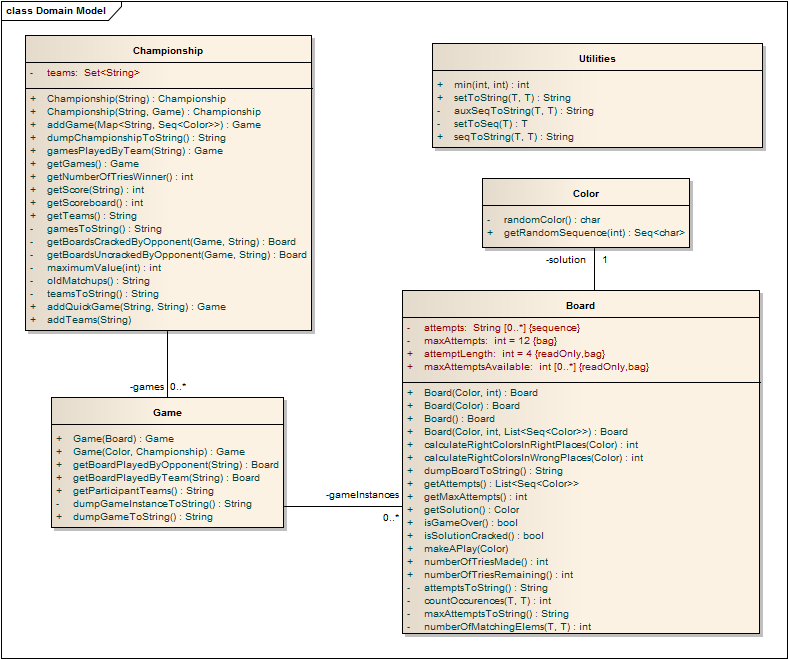
\includegraphics[scale=0.5]{../uml/model.png}    
  \caption{Diagrama UML com todas as classes do sistema.}
  \label{fig:diagrama_uml}
\end{figure}

Este diagrama foi obtido com a aplicação \emph{Overture Tools},
a partir da especificação formal em VDM++, e foram apenas reformulados
os tipos de dados não suportados pelo \emph{Enterprise Architect}.


\section{Definição completa das classes em VDM++}
\subsection{Color}

\begin{vdm_al}
class Color
  types
    public Color = char
    inv color == color in set {'b', 'g', 'r', 'o', 'y', 'm'};

  instance variables
    static public Colors : set of Color := {'b', 'g', 'r', 'o', 'y', 'm'};

  operations
    static public getRandomSequence: nat1 ==> seq1 of char
    getRandomSequence(length) == (

      if(length = 1) then
        return [randomColor()]
      else
        return [randomColor()] ^ getRandomSequence(length-1)

    )
    post len RESULT = length and
      forall color in set elems RESULT & color in set Colors;

    static private randomColor: () ==> char
    randomColor() == (

      ||(return 'b', return 'g', return 'r', return 'o', return 'y', return 'm';

    )
    post RESULT in set Colors;

end Color
\end{vdm_al}

\subsection{Utilities}

\begin{vdm_al}
class Utilities
  types
    public String = seq of char;

  functions

    -- Return the minimum of two values
    static public min : nat * nat -> nat
      min(a, b) ==
        if a <= b then a
        else b;


    static public seqToString[@T] : seq of [@T] * (@T -> String) -> String
    seqToString (sequence, printer) ==
      if sequence = [] then "[]"
      else "[" ^ auxSeqToString[@T](sequence, printer) ^ "]";


    static private auxSeqToString[@T] : seq1 of [@T] * (@T -> String) -> String
    auxSeqToString (sequence, printer) ==
      if len sequence = 1 then
        printer(hd sequence)
      else
        printer(hd sequence) ^ ", " ^ auxSeqToString[@T](tl sequence, printer);


    static private setToSeq[@T] : set of [@T] -> seq of [@T]
    setToSeq (s) ==
      if card s = 1 then
        let x in set s in [x]
      else
        let x in set s in
          [x] ^ setToSeq[@T](s\{x})
    pre s <> {}
    post forall element in set s & element in set elems RESULT;


    static public setToString[@T] : set of @T * (@T -> String) -> String
    setToString(s, printer) ==
      if s = {} then "{}"
      else "{" ^ auxSeqToString[@T](setToSeq[@T](s), printer) ^ "}";

end Utilities
\end{vdm_al}

\subsection{Board}
\begin{vdm_al}
class Board
  types
    public String = Utilities`String;

  instance variables
    private solution : seq1 of Color`Color;
    inv len solution = attemptLength;

    private attempts : seq of (seq1 of Color`Color) := [];
    inv forall attempt in set elems attempts & len attempt = attemptLength and
      len attempts <= maxAttempts;

    private maxAttempts : nat1 := 12;
    inv maxAttempts in set maxAttemptsAvailable;


  operations


    public Board : seq1 of Color`Color ==> Board
    Board (correctPlay) == (
      solution := correctPlay;
      attempts := [];
    )
    pre len correctPlay = attemptLength
    post solution = correctPlay and
      attempts = [];


    public Board : () ==> Board
    Board() == (

      solution := Color`getRandomSequence(attemptLength);
      attempts := [];

    )
    post len solution = attemptLength and attempts = [];


    public Board : seq1 of Color`Color * nat1 ==> Board
    Board (correctPlay, maxNumberOfTries) == (
      solution := correctPlay;
      maxAttempts := maxNumberOfTries;
    )
    pre len correctPlay = attemptLength and
      maxNumberOfTries in set maxAttemptsAvailable
    post solution = correctPlay and
      maxAttempts in set maxAttemptsAvailable;


    -- Constructor needed to recreate a board from the information of a file
    public Board : seq1 of Color`Color * nat1 * seq of (seq1 of Color`Color) ==> Board
    Board (correctPlay, maxNumberOfTries, savedAttempts) == (
      solution := correctPlay;
      maxAttempts := maxNumberOfTries;
      attempts := savedAttempts;
    )
    pre len correctPlay = attemptLength and
      maxNumberOfTries in set maxAttemptsAvailable and
      len savedAttempts <= maxNumberOfTries and
      forall attempt in set elems savedAttempts & len attempt = attemptLength

    post solution = correctPlay and
      maxAttempts = maxNumberOfTries and
      -- All elements of "attempts" need to be in the same position of the
      -- elements of "savedAttempts"
      numberOfMatchingElems[seq1 of Color`Color](attempts, savedAttempts) = len attempts;



    public numberOfTriesRemaining : () ==> nat
      numberOfTriesRemaining () == return maxAttempts - len attempts
    pre (len attempts) <= maxAttempts
    post RESULT = maxAttempts - len attempts;


    public numberOfTriesMade : () ==> nat
      numberOfTriesMade () == return len attempts
    post RESULT = len attempts;


    public makeAPlay : seq1 of Color`Color ==> ()
      makeAPlay (attempt) == attempts := attempts ^ [attempt]
    pre len attempt = attemptLength and
      not isGameOver()
    post attempts = attempts~ ^ [attempt];


    -- Return true if the correct code has been found
    public isSolutionCracked : () ==> bool
      isSolutionCracked () == return solution in set elems attempts
    post solution in set elems attempts => RESULT = true;


    public isGameOver : () ==> bool
      isGameOver () == return isSolutionCracked() or len attempts = maxAttempts
    post RESULT = (isSolutionCracked() or len attempts = maxAttempts);


    public calculateRightColorsInRightPlaces : seq of Color`Color ==> nat
      calculateRightColorsInRightPlaces (attempt) ==
        return numberOfMatchingElems[Color`Color](attempt, solution)
    pre len attempt = len solution
    post RESULT <= len solution;


    -- This formula is given in:
    -- http://mathworld.wolfram.com/Mastermind.html
    public calculateRightColorsInWrongPlaces : seq of Color`Color ==> nat
      calculateRightColorsInWrongPlaces (attempt) ==
      -- Just a temporary variable to hold the value of the sum expression
      -- (see previous URL)
        (dcl temp : nat := 0;
          for all color in set Color`Colors do
            temp := temp +
              Utilities`min(
                countOccurences[Color`Color](solution, color),
                countOccurences[Color`Color](attempt, color));
          return temp - calculateRightColorsInRightPlaces(attempt);
        )
    pre len attempt = len solution
    post RESULT <= len solution;


    public getSolution : () ==> seq1 of Color`Color
      getSolution () == return solution
    post RESULT = solution;


    public getAttempts : () ==> seq of (seq1 of Color`Color)
      getAttempts () == return attempts
    post RESULT = attempts;


    public getMaxAttempts : () ==> nat1
      getMaxAttempts () == return maxAttempts
    post RESULT = maxAttempts;



    -- Operators needed to write a Board to a file
    public dumpBoardToString : () ==> String
    dumpBoardToString () ==
      return "new Board(\"" ^ solution ^ "\", " ^ maxAttemptsToString()
        ^ ", " ^ attemptsToString() ^")";

    private attemptsToString : () ==> String
    attemptsToString () ==
      return Utilities`seqToString[seq1 of Color`Color](attempts,
        lambda x : String & "\"" ^ x ^ "\"");

    private maxAttemptsToString : () ==> String
    maxAttemptsToString () ==
      if maxAttempts = 8 then return "8"
      elseif maxAttempts = 10 then return "10"
      else return "12"
    pre maxAttempts = 8 or maxAttempts = 10 or maxAttempts = 12;


  functions

    -- Return the number of elements in the sequence that are a match both
    -- in value and in position. For example: [1,2,3,4,5] and [4,4,3,5,2]
    -- only has one element that matches both in value and in position (the
    -- element 3).
    private numberOfMatchingElems[@T] : seq of @T * seq of @T -> nat
      numberOfMatchingElems (firstSeq, secondSeq) ==
        if firstSeq = [] then
          0
        elseif hd firstSeq = hd secondSeq then
          1 + numberOfMatchingElems[@T](tl firstSeq, tl secondSeq)
        else
          numberOfMatchingElems[@T](tl firstSeq, tl secondSeq)
      pre (len firstSeq) = (len secondSeq)
      post firstSeq = [] => RESULT = 0;

    -- Return the number of times the element appears in the sequence
    private countOccurences[@T] : seq of @T * @T -> nat
      countOccurences (sequence, element) ==
        if sequence = [] then
          0
        elseif hd sequence = element then
          1 + countOccurences[@T](tl sequence, element)
        else
          countOccurences[@T](tl sequence, element)
      post sequence = [] => RESULT = 0;


  values
    public attemptLength : nat1 = 4;
    public maxAttemptsAvailable : set of nat1 = {8, 10, 12};

end Board
\end{vdm_al}

\subsection{Game}
\begin{vdm_al}
class Game

  types
    public String = Utilities`String;

  instance variables
    private gameInstances : map String to Board;
    inv card (dom gameInstances) = 2;

  operations

    public Game : map String to seq1 of Color`Color * Championship ==> Game
    Game (teamsSolutions, championship) == (

      let {team1, team2} = dom teamsSolutions in
        gameInstances := {team1 |-> new Board(teamsSolutions(team2)),
          team2 |-> new Board(teamsSolutions(team1))};

      )
    pre card (dom teamsSolutions) = 2 and
      forall team in set dom teamsSolutions &
        team in set championship.getTeams() and
      forall solution in set rng teamsSolutions &
        len solution = Board`attemptLength

    post forall team in set (dom gameInstances) &
      let opponentTeam = dom teamsSolutions \ {team} in
        {gameInstances(team).getSolution()} =
        rng (opponentTeam <: teamsSolutions);


    -- Constructor needed to recreate a game from the information of a file
    public Game : map String to Board ==> Game
    Game (storedGameInstances) ==
      gameInstances := storedGameInstances
    pre card (dom storedGameInstances) = 2
    post gameInstances = storedGameInstances;



    public getParticipantTeams : () ==> set of String
    getParticipantTeams () == return dom gameInstances
    post RESULT = dom gameInstances;


    public getBoardPlayedByTeam : String ==> Board
    getBoardPlayedByTeam (team) == return gameInstances(team)
    post RESULT = gameInstances(team);


    public getBoardPlayedByOpponent : String ==> Board
    getBoardPlayedByOpponent (team) ==
      let opponent in set (dom gameInstances)\{team}
      in
      return gameInstances(opponent)
    pre team in set (dom gameInstances)

    post RESULT in set rng gameInstances
      and {RESULT} = rng ({team} <-: gameInstances);


    -- Operators needed to write a Game to a file
    private dumpGameInstanceToString : () ==> String
    dumpGameInstanceToString () ==
      let {team1, team2} = dom gameInstances in
      return "{\"" ^ team1 ^ "\" |-> " ^ gameInstances(team1).dumpBoardToString() ^ ", "
        ^ "\"" ^ team2 ^ "\" |-> " ^ gameInstances(team2).dumpBoardToString() ^ "}"
    pre card (dom gameInstances) = 2;

    public dumpGameToString : () ==> String
    dumpGameToString () == return "new Game(" ^ dumpGameInstanceToString() ^ ")";

end Game
\end{vdm_al}

\subsection{Championship}
\begin{vdm_al}
class Championship

  types
    public String = Utilities`String;

  instance variables
    private teams : set of String;
    inv card teams >= 2 and (card teams) mod 2 = 0;

    private games : set of Game := {};
    inv forall game in set games & game.getParticipantTeams() subset teams;


  operations

    public Championship: set of String ==> Championship
    Championship(participants) == (

      teams := participants;

    )
    pre card participants >= 2 and (card participants) mod 2 = 0
    post teams = participants;


    -- Constructor needed to recreate a championship from the information of
    -- a file
    public Championship: set of String * set of Game ==> Championship
    Championship(participants, gamesPlayed) == (
      teams := participants;
      games := gamesPlayed
    )
    pre (card participants) >= 2 and (card participants) mod 2 = 0 and
      forall game in set gamesPlayed & game.getParticipantTeams() subset participants
    post teams = participants and games = gamesPlayed;


    public getTeams: () ==> set of String
    getTeams() == (

      return teams;

    )
    post RESULT = teams;


    public getGames: () ==> set of Game
    getGames() == (

      return games;

    )
    post RESULT = games;


    public addQuickGame: String * String ==> Game
    addQuickGame(team1, team2) == (

      dcl g : Game := new Game(
        {team1 |-> Color`getRandomSequence(Board`attemptLength),
          team2 |-> Color`getRandomSequence(Board`attemptLength)},
        self);

      games := games union {g};

      return g;

    )
    pre {team1, team2} subset teams and
      {team1, team2} not in set oldMatchups()
    post RESULT in set games;


    public addGame : map String to (seq of Color`Color) ==> Game
    addGame(teamsSolutions) == (

      dcl g : Game := new Game(teamsSolutions, self);

      games := games union {g};

      return g;

    )
    pre dom teamsSolutions subset teams and
      dom teamsSolutions not in set oldMatchups() and
      forall solution in set rng teamsSolutions & len solution = Board`attemptLength
    post RESULT in set games;


    public addTeams : set of String ==> ()
    addTeams(newTeams) == (

      teams := teams union newTeams;

    )
    pre (newTeams inter teams = {}) and (card newTeams) mod 2 = 0
    post teams = teams~ union newTeams;

    -- The codemaker gets one point for each guess a codebreaker makes. An
    -- extra point is earned by the codemaker if the codebreaker doesn't
    -- guess the pattern exactly in the last guess.
    public getScore : String ==> nat
    getScore (team) == (
      dcl gamesPlayed : set of Game := gamesPlayedByTeam(team),
        scoreByWinning : nat := 0,
        scoreByUndefeated : nat := 0;

        for board in getBoardsCrackedByOpponent(gamesPlayed, team) do
          scoreByWinning := scoreByWinning + board.numberOfTriesMade();

        for board in getBoardsUncrackedByOpponent(gamesPlayed, team) do
          scoreByUndefeated := scoreByUndefeated + board.numberOfTriesMade()+1;

        return scoreByWinning + scoreByUndefeated;

    )
    pre team in set teams;

    private oldMatchups : () ==> set of set of String
    oldMatchups () ==
      return {oldGames.getParticipantTeams() | oldGames in set games}
    post games = {} => RESULT = {};


    public gamesPlayedByTeam : String ==> set of Game
    gamesPlayedByTeam (team) ==
      return {game | game in set games & team in set game.getParticipantTeams()}
    post forall game in set RESULT
      & team in set game.getParticipantTeams();


    public getNumberOfTriesWinner : () ==> nat
    getNumberOfTriesWinner () ==
      let scoreBoard = getScoreboard()
      in
        return maximumValue(rng scoreBoard)
    pre let scoreboard = getScoreboard()
      in card dom (scoreboard :> {maximumValue(rng scoreboard)}) = 1;

    public getScoreboard : () ==> map String to nat
    getScoreboard () ==
      return { team |-> getScore(team) | team in set teams };


    -- Operators needed to write a Championship to a file
    private teamsToString : () ==> String
    teamsToString () ==
      return Utilities`setToString[String](teams,
        lambda x : String & "\"" ^ x ^ "\"");

    -- private gamesToString : () ==> String
    -- gamesToString () ==
    -- return Utilities`setToString[Game](games,
    --  lambda x : Game & x.dumpGameToString());
    --
    -- I wanted to implement "gamesToString" like this, but while it works
    -- with VDMTools, it does not work with Overture for some strange reason.
    -- Overture crashes with the following error:
    -- Illegal clone: java.lang.NullPointerException
    --
    -- Main 206: Error evaluating code
    -- Detailed Message: Illegal clone: java.lang.NullPointerException
    --
    -- So I needed to use the ugly implementation below, because it works in
    -- both systems.
    --  - Rolando

    private gamesToString : () ==> String
    gamesToString () ==
      if card games = 0 then return "{}"
      else (
        dcl return_value : String := "{",
          i : nat1 := 1;
        for all game in set games do
          if i < card games then (
            return_value := return_value  ^ " " ^ game.dumpGameToString() ^ ", ";
            i := i + 1;
          )
          else
            return_value := return_value ^ " " ^ game.dumpGameToString() ^ "}";

        return return_value;
      );

    public dumpChampionshipToString : () ==> String
    dumpChampionshipToString() ==
      return "new Championship(" ^ teamsToString() ^ ", " ^ gamesToString() ^ ")";


    functions

    private getBoardsUncrackedByOpponent : set of Game * String -> seq of Board
    getBoardsUncrackedByOpponent (games, team) ==
      if games = {} then []
      else let game in set games in
        let boardPlayedByOpponent = game.getBoardPlayedByOpponent(team) in
          if boardPlayedByOpponent.isGameOver() and
            not boardPlayedByOpponent.isSolutionCracked() then
              [boardPlayedByOpponent] ^ getBoardsUncrackedByOpponent(games\{game}, team)
          else
            getBoardsUncrackedByOpponent(games\{game}, team)

    post forall board in set elems RESULT & board.isGameOver() and not board.isSolutionCracked();


    private getBoardsCrackedByOpponent : set of Game * String -> seq of Board
    getBoardsCrackedByOpponent (games, team) ==
      if games = {} then []
      else let game in set games in
        let boardPlayedByOpponent = game.getBoardPlayedByOpponent(team) in
          if boardPlayedByOpponent.isGameOver() and
            boardPlayedByOpponent.isSolutionCracked() then
              [boardPlayedByOpponent] ^ getBoardsCrackedByOpponent(games\{game}, team)
          else
            getBoardsCrackedByOpponent(games\{game}, team)

    post forall board in set elems RESULT & board.isGameOver() and board.isSolutionCracked();

    
    private maximumValue : set of nat -> nat
    maximumValue (s) ==
      if card s = 1 then
        let x in set s in x
      else
        let x in set s in
          let max = maximumValue(s\{x}) in
            if x > max then
              x
            else
              max
    pre s <> {}
    post not exists element in set s & element > RESULT;

  
end Championship
\end{vdm_al}

\section{Informação de cobertura dos testes}

\subsection{Board}
\begin{vdm_al}
class Board
 types
  public String = Utilities`String;

 instance variables
  private solution : seq1 of Color`Color;
  inv len solution = attemptLength;

  private attempts : seq of (seq1 of Color`Color) := [];
  inv forall attempt in set elems attempts & len attempt = attemptLength and
   len attempts <= maxAttempts;

  private maxAttempts : nat1 := 12;
  inv maxAttempts in set maxAttemptsAvailable;


 operations


  public Board : seq1 of Color`Color ==> Board
  Board (correctPlay) == (
   solution := correctPlay;
   attempts := [];
  )
  pre len correctPlay = attemptLength
  post solution = correctPlay and
   attempts = [];


  public Board : () ==> Board
  Board() == (

   solution := Color`getRandomSequence(attemptLength);
   attempts := [];

  )
  post len solution = attemptLength and attempts = [];


  public Board : seq1 of Color`Color * nat1 ==> Board
  Board (correctPlay, maxNumberOfTries) == (
   solution := correctPlay;
   maxAttempts := maxNumberOfTries;
  )
  pre len correctPlay = attemptLength and
   maxNumberOfTries in set maxAttemptsAvailable
  post solution = correctPlay and
   maxAttempts in set maxAttemptsAvailable;


  -- Constructor needed to recreate a board from the information of a file
  public Board : seq1 of Color`Color * nat1 * seq of (seq1 of Color`Color) ==> Board
  Board (correctPlay, maxNumberOfTries, savedAttempts) == (
   solution := correctPlay;
   maxAttempts := maxNumberOfTries;
   attempts := savedAttempts;
  )
  pre len correctPlay = attemptLength and
   maxNumberOfTries in set maxAttemptsAvailable and
   len savedAttempts <= maxNumberOfTries and
   forall attempt in set elems savedAttempts & len attempt = attemptLength

  post solution = correctPlay and
   maxAttempts = maxNumberOfTries and
   -- All elements of "attempts" need to be in the same position of the
   -- elements of "savedAttempts"
   numberOfMatchingElems[seq1 of Color`Color](attempts, savedAttempts) = len attempts;



  public numberOfTriesRemaining : () ==> nat
   numberOfTriesRemaining () == return maxAttempts - len attempts
  pre (len attempts) <= maxAttempts
  post RESULT = maxAttempts - len attempts;


  public numberOfTriesMade : () ==> nat
   numberOfTriesMade () == return len attempts
  post RESULT = len attempts;


  public makeAPlay : seq1 of Color`Color ==> ()
   makeAPlay (attempt) == attempts := attempts ^ [attempt]
  pre len attempt = attemptLength and
   not isGameOver()
  post attempts = attempts~ ^ [attempt];


  -- Return true if the correct code has been found
  public isSolutionCracked : () ==> bool
   isSolutionCracked () == return solution in set elems attempts
  post solution in set elems attempts => RESULT = true;


  public isGameOver : () ==> bool
   isGameOver () == return isSolutionCracked() or len attempts = maxAttempts
  post RESULT = (isSolutionCracked() or len attempts = maxAttempts);


  public calculateRightColorsInRightPlaces : seq of Color`Color ==> nat
   calculateRightColorsInRightPlaces (attempt) ==
    return numberOfMatchingElems[Color`Color](attempt, solution)
  pre len attempt = len solution
  post RESULT <= len solution;


  -- This formula is given in:
  -- http://mathworld.wolfram.com/Mastermind.html
  public calculateRightColorsInWrongPlaces : seq of Color`Color ==> nat
   calculateRightColorsInWrongPlaces (attempt) ==
   -- Just a temporary variable to hold the value of the sum expression
   -- (see previous URL)
    (dcl temp : nat := 0;
     for all color in set Color`Colors do
      temp := temp +
       Utilities`min(
        countOccurences[Color`Color](solution, color),
        countOccurences[Color`Color](attempt, color));
     return temp - calculateRightColorsInRightPlaces(attempt);
    )
  pre len attempt = len solution
  post RESULT <= len solution;


  public getSolution : () ==> seq1 of Color`Color
   getSolution () == return solution
  post RESULT = solution;


  public getAttempts : () ==> seq of (seq1 of Color`Color)
   getAttempts () == return attempts
  post RESULT = attempts;


  public getMaxAttempts : () ==> nat1
   getMaxAttempts () == return maxAttempts
  post RESULT = maxAttempts;



  -- Operators needed to write a Board to a file
  public dumpBoardToString : () ==> String
  dumpBoardToString () ==
   return "new Board(\"" ^ solution ^ "\", " ^ maxAttemptsToString()
    ^ ", " ^ attemptsToString() ^")";

  private attemptsToString : () ==> String
  attemptsToString () ==
   return Utilities`seqToString[seq1 of Color`Color](attempts,
    lambda x : String & "\"" ^ x ^ "\"");

  private maxAttemptsToString : () ==> String
  maxAttemptsToString () ==
   if maxAttempts = 8 then return "8"
   elseif maxAttempts = 10 then return "10"
   else return "12"
  pre maxAttempts = 8 or maxAttempts = 10 or maxAttempts = 12;


 functions

  -- Return the number of elements in the sequence that are a match both
  -- in value and in position. For example: [1,2,3,4,5] and [4,4,3,5,2]
  -- only has one element that matches both in value and in position (the
  -- element 3).
  private numberOfMatchingElems[@T] : seq of @T * seq of @T -> nat
   numberOfMatchingElems (firstSeq, secondSeq) ==
    if firstSeq = [] then
     0
    elseif hd firstSeq = hd secondSeq then
     1 + numberOfMatchingElems[@T](tl firstSeq, tl secondSeq)
    else
     numberOfMatchingElems[@T](tl firstSeq, tl secondSeq)
   pre (len firstSeq) = (len secondSeq)
   post firstSeq = [] => RESULT = 0;

  -- Return the number of times the element appears in the sequence
  private countOccurences[@T] : seq of @T * @T -> nat
   countOccurences (sequence, element) ==
    if sequence = [] then
     0
    elseif hd sequence = element then
     1 + countOccurences[@T](tl sequence, element)
    else
     countOccurences[@T](tl sequence, element)
   post sequence = [] => RESULT = 0;


 values
  public attemptLength : nat1 = 4;
  public maxAttemptsAvailable : set of nat1 = {8, 10, 12};

end Board
\end{vdm_al}
\bigskip
\begin{longtable}{|l|r|r|}
\hline
Function or operation & Coverage & Calls \\
\hline
\hline
Board & 100.0\% & 94 \\
\hline
attemptsToString & 100.0\% & 94 \\
\hline
calculateRightColorsInRightPlaces & 100.0\% & 42 \\
\hline
calculateRightColorsInWrongPlaces & 100.0\% & 24 \\
\hline
countOccurences & 100.0\% & 1440 \\
\hline
dumpBoardToString & 100.0\% & 94 \\
\hline
getAttempts & 100.0\% & 626 \\
\hline
getMaxAttempts & 100.0\% & 188 \\
\hline
getSolution & 100.0\% & 304 \\
\hline
isGameOver & 100.0\% & 562 \\
\hline
isSolutionCracked & 100.0\% & 1274 \\
\hline
makeAPlay & 100.0\% & 350 \\
\hline
maxAttemptsToString & 100.0\% & 94 \\
\hline
numberOfMatchingElems & 100.0\% & 476 \\
\hline
numberOfTriesMade & 100.0\% & 52 \\
\hline
numberOfTriesRemaining & 100.0\% & 24 \\
\hline
\hline
Board.vdmpp & 100.0\% & 5738 \\
\hline
\end{longtable}


\subsection{BoardTest}
\begin{vdm_al}
class BoardTest
 types
  public String = Utilities`String;

 operations
 static public AssertTrue : bool ==> ()
  AssertTrue(a) == return
    pre a;


 static public runAllTests : () ==> ()
  runAllTests () == (
   testGoodGame1();
   testGoodGame2();
   testGoodGame3();
   testGoodGame4();
   testGoodGame5();
   testRightColorsInRightPlaces();
   testRightColorsInWrongPlaces();
   testReadSimpleBoardFromFile();
   testReadMaxAttemptsChangedBoardFromFile();
   testReadNormalBoardFromFile();
  );


 static public testGoodGame1 : () ==> ()
 testGoodGame1 () ==
 ( dcl b : Board := new Board(['b', 'b', 'b', 'b']);
  b.makeAPlay(['b', 'b', 'b', 'b']);
  AssertTrue(b.isSolutionCracked());
 );


 static public testGoodGame2 : () ==> ()
 testGoodGame2 () ==
 ( dcl b : Board := new Board(['b', 'b', 'b', 'b']);
  AssertTrue(b.numberOfTriesRemaining() = 12);
  b.makeAPlay(['b', 'b', 'b', 'b']);
  AssertTrue(b.numberOfTriesRemaining() = 11);
 );


 static public testGoodGame3 : () ==> ()
 testGoodGame3 () ==
 ( dcl b : Board := new Board(['b', 'r', 'y', 'o']);
  AssertTrue(b.numberOfTriesMade() = 0);
  b.makeAPlay(['b', 'b', 'b', 'b']);
  AssertTrue(b.numberOfTriesMade() = 1);
 );


 static public testGoodGame4 : () ==> ()
 testGoodGame4 () ==
 ( dcl b : Board := new Board(['b', 'r', 'y', 'o'], 10);
  AssertTrue(b.numberOfTriesRemaining() = 10);
  b.makeAPlay(['b', 'b', 'b', 'b']);
  AssertTrue(b.numberOfTriesRemaining() = 9);

 );


 static public testGoodGame5 : () ==> ()
 testGoodGame5 () ==
  let b = new Board()
   in
   AssertTrue (len b.getSolution() = Board`attemptLength);


 static public testRightColorsInRightPlaces : () ==> ()
 testRightColorsInRightPlaces () ==
  let b = new Board(['b', 'b', 'b', 'b']),
   solutionToValue = {
    ['b', 'b', 'r', 'o'] |-> 2,
    ['r', 'r', 'r', 'o'] |-> 0,
    ['b', 'b', 'b', 'b'] |-> 4
   } in
   AssertTrue(forall solution in set (dom solutionToValue)
    & b.calculateRightColorsInRightPlaces(solution) = solutionToValue(solution));


 static public testRightColorsInWrongPlaces : () ==> ()
 testRightColorsInWrongPlaces () ==
  let b = new Board(['b', 'r', 'y', 'o']),
   solutionToValue = {
    ['r', 'm', 'm', 'm'] |-> 1,
    ['m', 'r', 'm', 'm'] |-> 0,
    ['m', 'r', 'm', 'y'] |-> 1,
    ['y', 'm', 'm', 'y'] |-> 1
   } in
   AssertTrue(forall solution in set (dom solutionToValue)
    & b.calculateRightColorsInWrongPlaces(solution) = solutionToValue(solution));


 static public testReadSimpleBoardFromFile : () ==> ()
 testReadSimpleBoardFromFile () == (
  writeAndReadBoardFromFile("simpleBoard1.txt", new Board("bbbb"));
  writeAndReadBoardFromFile("simpleBoard2.txt", new Board("rbmg"));
 );

 static public testReadMaxAttemptsChangedBoardFromFile : () ==> ()
 testReadMaxAttemptsChangedBoardFromFile () == (
  writeAndReadBoardFromFile("maxAttemptsBoard1.txt", new Board("bbbb", 8));
  writeAndReadBoardFromFile("maxAttemptsBoard2.txt", new Board("bbbb", 10));
  writeAndReadBoardFromFile("maxAttemptsBoard3.txt", new Board("bbbb", 12));
 );

 static public testReadNormalBoardFromFile : () ==> ()
 testReadNormalBoardFromFile () == (
  dcl board1 : Board := new Board("bbbb"),
   board2 : Board := new Board("bryo"),
   board3 : Board := new Board("rgmb", 8);

   board1.makeAPlay("rgrg");
   board1.makeAPlay("gggg");
   board1.makeAPlay("bbbb");

   board2.makeAPlay("mmmm");
   board2.makeAPlay("bgbg");
   board2.makeAPlay("ryry");

   -- Perform the max ammount of plays (in this case 8)
   board3.makeAPlay("ogrm");
   board3.makeAPlay("gbry");
   board3.makeAPlay("romo");
   board3.makeAPlay("yrry");
   board3.makeAPlay("roby");
   board3.makeAPlay("gmbr");
   board3.makeAPlay("gomy");
   board3.makeAPlay("ybyr");

   writeAndReadBoardFromFile("normalBoard1.txt", board1);
   writeAndReadBoardFromFile("normalBoard2.txt", board2);
   writeAndReadBoardFromFile("normalBoard3.txt", board3);
  );


 static private writeAndReadBoardFromFile : String * Board ==> ()
 writeAndReadBoardFromFile (filename, board) == (
  dcl io : IO := new IO(),
  writeSuccess : bool := io.fecho(filename, board.dumpBoardToString(), <start>);

  -- Check if the file was correctly created
  AssertTrue(writeSuccess = true);

  let mk_(readSuccess, boardFromDisk) = io.freadval[Board](filename) in (
   -- Check if the file was correctly read
   AssertTrue(readSuccess = true);

   -- Perform consistency checks
   AssertTrue(board.getSolution() = boardFromDisk.getSolution());
   AssertTrue(board.getMaxAttempts() = boardFromDisk.getMaxAttempts());

   AssertTrue(len board.getAttempts() = len boardFromDisk.getAttempts());

   -- Since the attempts are a 'seq', check if the order of its elements
   -- stays the same
   AssertTrue(forall i in set inds board.getAttempts() &
    board.getAttempts()(i) = boardFromDisk.getAttempts()(i));
  )
 );

end BoardTest
\end{vdm_al}
\bigskip
\begin{longtable}{|l|r|r|}
\hline
Function or operation & Coverage & Calls \\
\hline
\hline
AssertTrue & 100.0\% & 348 \\
\hline
runAllTests & 100.0\% & 6 \\
\hline
testGoodGame1 & 100.0\% & 6 \\
\hline
testGoodGame2 & 100.0\% & 6 \\
\hline
testGoodGame3 & 100.0\% & 6 \\
\hline
testGoodGame4 & 100.0\% & 6 \\
\hline
testGoodGame5 & 100.0\% & 6 \\
\hline
testReadMaxAttemptsChangedBoardFromFile & 100.0\% & 6 \\
\hline
testReadNormalBoardFromFile & 100.0\% & 6 \\
\hline
testReadSimpleBoardFromFile & 100.0\% & 6 \\
\hline
testRightColorsInRightPlaces & 100.0\% & 6 \\
\hline
testRightColorsInWrongPlaces & 100.0\% & 6 \\
\hline
writeAndReadBoardFromFile & 100.0\% & 48 \\
\hline
\hline
BoardTest.vdmpp & 100.0\% & 462 \\
\hline
\end{longtable}


\subsection{Championship}
\begin{vdm_al}
class Championship

 types
  public String = Utilities`String;

 instance variables
  private teams : set of String;
  inv card teams >= 2 and (card teams) mod 2 = 0;

  private games : set of Game := {};
  inv forall game in set games & game.getParticipantTeams() subset teams;


 operations

  public Championship: set of String ==> Championship
  Championship(participants) == (

   teams := participants;

  )
  pre card participants >= 2 and (card participants) mod 2 = 0
  post teams = participants;


  -- Constructor needed to recreate a championship from the information of
  -- a file
  public Championship: set of String * set of Game ==> Championship
  Championship(participants, gamesPlayed) == (
   teams := participants;
   games := gamesPlayed
  )
  pre (card participants) >= 2 and (card participants) mod 2 = 0 and
   forall game in set gamesPlayed & game.getParticipantTeams() subset participants
  post teams = participants and games = gamesPlayed;


  public getTeams: () ==> set of String
  getTeams() == (

   return teams;

  )
  post RESULT = teams;


  public getGames: () ==> set of Game
  getGames() == (

   return games;

  )
  post RESULT = games;


  public addQuickGame: String * String ==> Game
  addQuickGame(team1, team2) == (

   dcl g : Game := new Game(
    {team1 |-> Color`getRandomSequence(Board`attemptLength),
     team2 |-> Color`getRandomSequence(Board`attemptLength)},
    self);

   games := games union {g};

   return g;

  )
  pre {team1, team2} subset teams and
   {team1, team2} not in set oldMatchups()
  post RESULT in set games;


  public addGame : map String to (seq of Color`Color) ==> Game
  addGame(teamsSolutions) == (

   dcl g : Game := new Game(teamsSolutions, self);

   games := games union {g};

   return g;

  )
  pre dom teamsSolutions subset teams and
   dom teamsSolutions not in set oldMatchups() and
   forall solution in set rng teamsSolutions & len solution = Board`attemptLength
  post RESULT in set games;


  public addTeams : set of String ==> ()
  addTeams(newTeams) == (

   teams := teams union newTeams;

  )
  pre (newTeams inter teams = {}) and (card newTeams) mod 2 = 0
  post teams = teams~ union newTeams;

  -- The codemaker gets one point for each guess a codebreaker makes. An
  -- extra point is earned by the codemaker if the codebreaker doesn't
  -- guess the pattern exactly in the last guess.
  public getScore : String ==> nat
  getScore (team) == (
   dcl gamesPlayed : set of Game := gamesPlayedByTeam(team),
    scoreByWinning : nat := 0,
    scoreByUndefeated : nat := 0;

    for board in getBoardsCrackedByOpponent(gamesPlayed, team) do
     scoreByWinning := scoreByWinning + board.numberOfTriesMade();

    for board in getBoardsUncrackedByOpponent(gamesPlayed, team) do
     scoreByUndefeated := scoreByUndefeated + board.numberOfTriesMade()+1;

    return scoreByWinning + scoreByUndefeated;

  )
  pre team in set teams;

  private oldMatchups : () ==> set of set of String
  oldMatchups () ==
   return {oldGames.getParticipantTeams() | oldGames in set games}
  post games = {} => RESULT = {};


  public gamesPlayedByTeam : String ==> set of Game
  gamesPlayedByTeam (team) ==
   return {game | game in set games & team in set game.getParticipantTeams()}
  post forall game in set RESULT
   & team in set game.getParticipantTeams();


  public getNumberOfTriesWinner : () ==> nat
  getNumberOfTriesWinner () ==
   let scoreBoard = getScoreboard()
   in
    return maximumValue(rng scoreBoard)
  pre let scoreboard = getScoreboard()
   in card dom (scoreboard :> {maximumValue(rng scoreboard)}) = 1;

  public getScoreboard : () ==> map String to nat
  getScoreboard () ==
   return { team |-> getScore(team) | team in set teams };


  -- Operators needed to write a Championship to a file
  private teamsToString : () ==> String
  teamsToString () ==
   return Utilities`setToString[String](teams,
    lambda x : String & "\"" ^ x ^ "\"");

  -- private gamesToString : () ==> String
  -- gamesToString () ==
  -- return Utilities`setToString[Game](games,
  --  lambda x : Game & x.dumpGameToString());
  --
  -- I wanted to implement "gamesToString" like this, but while it works
  -- with VDMTools, it does not work with Overture for some strange reason.
  -- Overture crashes with the following error:
  -- Illegal clone: java.lang.NullPointerException
  --
  -- Main 206: Error evaluating code
  -- Detailed Message: Illegal clone: java.lang.NullPointerException
  --
  -- So I needed to use the ugly implementation below, because it works in
  -- both systems.
  --  - Rolando

  private gamesToString : () ==> String
  gamesToString () ==
   if card games = 0 then return "{}"
   else (
    dcl return_value : String := "{",
     i : nat1 := 1;
    for all game in set games do
     if i < card games then (
      return_value := return_value  ^ " " ^ game.dumpGameToString() ^ ", ";
      i := i + 1;
     )
     else
      return_value := return_value ^ " " ^ game.dumpGameToString() ^ "}";

    return return_value;
   );

  public dumpChampionshipToString : () ==> String
  dumpChampionshipToString() ==
   return "new Championship(" ^ teamsToString() ^ ", " ^ gamesToString() ^ ")";


  functions

  private getBoardsUncrackedByOpponent : set of Game * String -> seq of Board
  getBoardsUncrackedByOpponent (games, team) ==
   if games = {} then []
   else let game in set games in
    let boardPlayedByOpponent = game.getBoardPlayedByOpponent(team) in
     if boardPlayedByOpponent.isGameOver() and
      not boardPlayedByOpponent.isSolutionCracked() then
       [boardPlayedByOpponent] ^ getBoardsUncrackedByOpponent(games\{game}, team)
     else
      getBoardsUncrackedByOpponent(games\{game}, team)

  post forall board in set elems RESULT & board.isGameOver() and not board.isSolutionCracked();


  private getBoardsCrackedByOpponent : set of Game * String -> seq of Board
  getBoardsCrackedByOpponent (games, team) ==
   if games = {} then []
   else let game in set games in
    let boardPlayedByOpponent = game.getBoardPlayedByOpponent(team) in
     if boardPlayedByOpponent.isGameOver() and
      boardPlayedByOpponent.isSolutionCracked() then
       [boardPlayedByOpponent] ^ getBoardsCrackedByOpponent(games\{game}, team)
     else
      getBoardsCrackedByOpponent(games\{game}, team)

  post forall board in set elems RESULT & board.isGameOver() and board.isSolutionCracked();

  
  private maximumValue : set of nat -> nat
  maximumValue (s) ==
   if card s = 1 then
    let x in set s in x
   else
    let x in set s in
     let max = maximumValue(s\{x}) in
      if x > max then
       (*@\notcovered{x}@*)
      else
       max
  pre s <> {}
  post not exists element in set s & element > RESULT;

 
end Championship
\end{vdm_al}
\bigskip
\begin{longtable}{|l|r|r|}
\hline
Function or operation & Coverage & Calls \\
\hline
\hline
Championship & 100.0\% & 24 \\
\hline
addGame & 100.0\% & 43 \\
\hline
addQuickGame & 100.0\% & 6 \\
\hline
addTeams & 100.0\% & 6 \\
\hline
dumpChampionshipToString & 100.0\% & 19 \\
\hline
gamesPlayedByTeam & 100.0\% & 98 \\
\hline
gamesToString & 100.0\% & 19 \\
\hline
getBoardsCrackedByOpponent & 100.0\% & 136 \\
\hline
getBoardsUncrackedByOpponent & 100.0\% & 136 \\
\hline
getGames & 100.0\% & 101 \\
\hline
getNumberOfTriesWinner & 100.0\% & 6 \\
\hline
getScore & 100.0\% & 98 \\
\hline
getScoreboard & 100.0\% & 10 \\
\hline
getTeams & 100.0\% & 194 \\
\hline
maximumValue & 96.7\% & 32 \\
\hline
oldMatchups & 100.0\% & 49 \\
\hline
teamsToString & 100.0\% & 19 \\
\hline
\hline
Championship.vdmpp & 99.7\% & 996 \\
\hline
\end{longtable}



Pensamos que a razão pela qual a função ``maximumValue'' não se
encontra testada a 100\% deve-se à natureza não determinística da
iteração em variáveis do tipo \texttt{set} o que levou a que nunca
fosse escolhido um ``X'' que fizesse com que o código seguisse aquele
caminho.

Assumimos que se a função ``maximumValue'' fosse executada um elevado
número de vezes, que este caminho de código seria também executado.

\subsection{ChampionshipTest}
\begin{vdm_al}
class ChampionshipTest
 types
  public String = Utilities`String;

 operations
 static public AssertTrue : bool ==> ()
  AssertTrue(a) == return
 pre a;


 static public runAllTests : () ==> ()
 runAllTests () == (
  testNewChampionship1();
  testNewChampionship2();
  testAddGame1();
  testAddGame2();
  testCalculateScores();
  testReadSimpleChampionshipFromFile();
  testReadChampionshipWithGamesFromFile();
  testReadNormalChampionshipFromFile();
 );


 static public testNewChampionship1 : () ==> ()
 testNewChampionship1() ==
  ( dcl c : Championship := new Championship({"Spartans","Romans"});

   AssertTrue(card c.getTeams() = 2);
   AssertTrue(c.getTeams() = {"Spartans", "Romans"});
   AssertTrue(c.getScore("Spartans") = 0);
   AssertTrue(c.getScore("Romans") = 0);

  );


 static public testNewChampionship2 : () ==> ()
 testNewChampionship2() ==
  ( dcl c : Championship := new Championship({"Spartans", "Romans"});

   AssertTrue(card c.getTeams() = 2);
   AssertTrue(c.getTeams() = {"Spartans", "Romans"});
   c.addTeams({"Gauls", "Greeks"});
   AssertTrue(card c.getTeams() = 4);
   AssertTrue({"Gauls", "Greeks"} subset c.getTeams());

  );


 static public testAddGame1 : () ==> ()
 testAddGame1() ==
  ( dcl c : Championship := new Championship({"Spartans", "Romans"}),
   g  : Game  := c.addQuickGame("Spartans","Romans"),
   b1 : Board := g.getBoardPlayedByTeam("Spartans"),
   b2 : Board := g.getBoardPlayedByTeam("Romans");

   AssertTrue((g.getParticipantTeams() subset c.getTeams()));
   AssertTrue(g in set c.getGames());

   AssertTrue(b1.isSolutionCracked() = false);
   AssertTrue(b2.isSolutionCracked() = false);

  );


 static public testAddGame2 : () ==> ()
 testAddGame2() ==
  ( dcl solSpartans : seq1 of Color`Color := ['b', 'b', 'r', 'b'],
   solRomans : seq1 of Color`Color := ['r', 'r', 'b', 'r'],
   c : Championship := new Championship({"Spartans", "Romans"}),
   g : Game := c.addGame({"Spartans" |-> solSpartans, "Romans" |-> solRomans}),
   b1 : Board := g.getBoardPlayedByTeam("Spartans"),
   b2 : Board := g.getBoardPlayedByTeam("Romans");

   AssertTrue((g.getParticipantTeams() subset c.getTeams()));

   AssertTrue(b1.isSolutionCracked() = false);
   AssertTrue(b2.isSolutionCracked() = false);

   AssertTrue(b1.getSolution() = solRomans);
   AssertTrue(b2.getSolution() = solSpartans);

   AssertTrue(c.getScore("Spartans") = 0);
   AssertTrue(c.getScore("Romans") = 0);

  );


 static public testCalculateScores : () ==> ()
 testCalculateScores () == (
   dcl c1 : Championship := new Championship({"lorem", "ipsum", "foo", "bar"}),
   g1 : Game := c1.addGame({"lorem" |-> "bbbb", "ipsum" |-> "rrrr"}),
   g2 : Game := c1.addGame({"foo" |-> "rgrg", "bar" |-> "mymy"});

   g1.getBoardPlayedByTeam("lorem").makeAPlay("rggg");

   -- "ipsum" cracks the code in 5 tries so "lorem" gains 5 points
   g1.getBoardPlayedByTeam("ipsum").makeAPlay("bbrg");
   g1.getBoardPlayedByTeam("ipsum").makeAPlay("mrob");
   g1.getBoardPlayedByTeam("ipsum").makeAPlay("bobm");
   g1.getBoardPlayedByTeam("ipsum").makeAPlay("bgbm");
   g1.getBoardPlayedByTeam("ipsum").makeAPlay("bbbb");

   -- "foo" can't crack this board, so "bar" gains 13 points
   g2.getBoardPlayedByTeam("foo").makeAPlay("ggym");
   g2.getBoardPlayedByTeam("foo").makeAPlay("yomo");
   g2.getBoardPlayedByTeam("foo").makeAPlay("ggbb");
   g2.getBoardPlayedByTeam("foo").makeAPlay("royy");
   g2.getBoardPlayedByTeam("foo").makeAPlay("mgby");
   g2.getBoardPlayedByTeam("foo").makeAPlay("gror");
   g2.getBoardPlayedByTeam("foo").makeAPlay("grgr");
   g2.getBoardPlayedByTeam("foo").makeAPlay("grrr");
   g2.getBoardPlayedByTeam("foo").makeAPlay("grgr");
   g2.getBoardPlayedByTeam("foo").makeAPlay("ggrr");
   g2.getBoardPlayedByTeam("foo").makeAPlay("grgg");
   g2.getBoardPlayedByTeam("foo").makeAPlay("yyyy");

   g2.getBoardPlayedByTeam("bar").makeAPlay("mbrb");
   g2.getBoardPlayedByTeam("bar").makeAPlay("bybb");
   g2.getBoardPlayedByTeam("bar").makeAPlay("ggry");
   g2.getBoardPlayedByTeam("bar").makeAPlay("rmom");

   AssertTrue(c1.getScore("lorem") = 5);
   AssertTrue(c1.getScore("ipsum") = 0);
   AssertTrue(c1.getScore("foo") = 0);
   AssertTrue(c1.getScore("bar") = 13);

   AssertTrue(c1.getNumberOfTriesWinner() = 13);
  );


 static public testReadSimpleChampionshipFromFile : () ==> ()
 testReadSimpleChampionshipFromFile () == (
  writeAndReadChampionshipFromFile("simpleChampionship1.txt",
   new Championship({"lorem", "ipsum"}));
  writeAndReadChampionshipFromFile("simpleChampionship2.txt",
   new Championship({"lorem", "ipsum", "foo", "bar"}));
 );

 static public testReadChampionshipWithGamesFromFile : () ==> ()
 testReadChampionshipWithGamesFromFile () == (
  dcl c1 : Championship := new Championship({"lorem", "ipsum"}),
   c2 : Championship := new Championship({"lorem", "ipsum", "foo", "bar"}),
   g1 : Game := c1.addGame({"lorem" |-> "bbbb", "ipsum" |-> "rrrr"}),
   g2 : Game := c2.addGame({"lorem" |-> "bbbb", "ipsum" |-> "rrrr"}),
   g3 : Game := c2.addGame({"foo" |-> "rgrg", "ipsum" |-> "mymy"});

   writeAndReadChampionshipFromFile("championshipWithGames1.txt", c1);
   writeAndReadChampionshipFromFile("championshipWithGames2.txt", c2);
  );

 static public testReadNormalChampionshipFromFile : () ==> ()
 testReadNormalChampionshipFromFile () == (
  dcl c1 : Championship := new Championship({"lorem", "ipsum", "foo", "bar"}),
   g1 : Game := c1.addGame({"lorem" |-> "bbbb", "ipsum" |-> "rrrr"}),
   g2 : Game := c1.addGame({"foo" |-> "rgrg", "bar" |-> "mymy"});

   g1.getBoardPlayedByTeam("lorem").makeAPlay("rrrr");

   g1.getBoardPlayedByTeam("ipsum").makeAPlay("bbrg");
   g1.getBoardPlayedByTeam("ipsum").makeAPlay("mrob");
   g1.getBoardPlayedByTeam("ipsum").makeAPlay("bobm");
   g1.getBoardPlayedByTeam("ipsum").makeAPlay("bgbm");
   g1.getBoardPlayedByTeam("ipsum").makeAPlay("bbbb");

   g2.getBoardPlayedByTeam("foo").makeAPlay("ggym");
   g2.getBoardPlayedByTeam("foo").makeAPlay("yomo");
   g2.getBoardPlayedByTeam("foo").makeAPlay("ggbb");
   g2.getBoardPlayedByTeam("foo").makeAPlay("royy");
   g2.getBoardPlayedByTeam("foo").makeAPlay("mgby");
   g2.getBoardPlayedByTeam("foo").makeAPlay("gror");
   g2.getBoardPlayedByTeam("foo").makeAPlay("grgr");
   g2.getBoardPlayedByTeam("foo").makeAPlay("grrr");
   g2.getBoardPlayedByTeam("foo").makeAPlay("grgr");
   g2.getBoardPlayedByTeam("foo").makeAPlay("ggrr");
   g2.getBoardPlayedByTeam("foo").makeAPlay("grgg");
   g2.getBoardPlayedByTeam("foo").makeAPlay("yyyy");

   g2.getBoardPlayedByTeam("bar").makeAPlay("mbrb");
   g2.getBoardPlayedByTeam("bar").makeAPlay("bybb");
   g2.getBoardPlayedByTeam("bar").makeAPlay("ggry");
   g2.getBoardPlayedByTeam("bar").makeAPlay("rmom");

   writeAndReadChampionshipFromFile("normalChampionship1.txt", c1);
  );

 static private writeAndReadChampionshipFromFile : String * Championship ==> ()
 writeAndReadChampionshipFromFile (filename, championship) == (
  dcl io : IO := new IO(),
  writeSuccess : bool := io.fecho(filename, championship.dumpChampionshipToString(), <start>);

  -- Check if the file was correctly created
  AssertTrue(writeSuccess = true);

  let mk_(readSuccess, championshipFromDisk) = io.freadval[Championship](filename) in (
   -- Check if the file was correctly read
   AssertTrue(readSuccess = true);

   -- Perform consistency checks
   AssertTrue(championship.getTeams() = championshipFromDisk.getTeams());

   AssertTrue(card championship.getGames() = card championshipFromDisk.getGames());
   AssertTrue(forall i in set championship.getGames() &
    exists1 j in set championshipFromDisk.getGames() &
    isSameGame(i, j));
   )
  );


 functions

 static private isSameGame : Game * Game -> bool
 isSameGame (game1, game2) ==
  -- Both games must have the same teams playing
  game1.getParticipantTeams() = game2.getParticipantTeams() and

  -- The board played by each team must be the same
  forall team in set game1.getParticipantTeams() &
   isSameBoard(game1.getBoardPlayedByTeam(team),
    game2.getBoardPlayedByTeam(team));


 static private isSameBoard : Board * Board -> bool
 isSameBoard (board1, board2) ==
  -- Both boards must have he same solution
  board1.getSolution() = board2.getSolution() and

  -- Both boards must have the same number of maximum attempts
  board1.getMaxAttempts() = board2.getMaxAttempts() and

  -- Both boards must have the same number of attempts
  len board1.getAttempts() = len board2.getAttempts() and

  -- Those attempts must be the same in both boards
  forall i in set inds board1.getAttempts() &
   board1.getAttempts()(i) = board2.getAttempts()(i);

end ChampionshipTest
\end{vdm_al}
\bigskip
\begin{longtable}{|l|r|r|}
\hline
Function or operation & Coverage & Calls \\
\hline
\hline
AssertTrue & 100.0\% & 263 \\
\hline
isSameBoard & 100.0\% & 80 \\
\hline
isSameGame & 100.0\% & 72 \\
\hline
runAllTests & 100.0\% & 6 \\
\hline
testAddGame1 & 100.0\% & 6 \\
\hline
testAddGame2 & 100.0\% & 6 \\
\hline
testCalculateScores & 100.0\% & 6 \\
\hline
testNewChampionship1 & 100.0\% & 6 \\
\hline
testNewChampionship2 & 100.0\% & 6 \\
\hline
testReadChampionshipWithGamesFromFile & 100.0\% & 5 \\
\hline
testReadNormalChampionshipFromFile & 100.0\% & 5 \\
\hline
testReadSimpleChampionshipFromFile & 100.0\% & 5 \\
\hline
writeAndReadChampionshipFromFile & 100.0\% & 20 \\
\hline
\hline
ChampionshipTest.vdmpp & 100.0\% & 486 \\
\hline
\end{longtable}



\subsection{Color}
\begin{vdm_al}
class Color
 types
  public Color = char
  inv color == (*@\notcovered{color}@*) (*@\notcovered{in}@*) set (*@\notcovered{\{}@*)(*@\notcovered{'}@*)b', (*@\notcovered{'}@*)g', (*@\notcovered{'}@*)r', (*@\notcovered{'}@*)o', (*@\notcovered{'}@*)y', (*@\notcovered{'}@*)m'};

 instance variables
  static public Colors : set of Color := {'b', 'g', 'r', 'o', 'y', 'm'};

 operations
  static public getRandomSequence: nat1 ==> seq1 of char
  getRandomSequence(length) == (

   if(length = 1) then
    return [randomColor()]
   else
    return [randomColor()] ^ getRandomSequence(length-1)

  )
  post len RESULT = length and
   forall color in set elems RESULT & color in set Colors;

  static private randomColor: () ==> char
  randomColor() == (

   ||(return 'b', (*@\notcovered{return}@*) (*@\notcovered{'}@*)g', (*@\notcovered{return}@*) (*@\notcovered{'}@*)r', (*@\notcovered{return}@*) (*@\notcovered{'}@*)o', (*@\notcovered{return}@*) (*@\notcovered{'}@*)y', (*@\notcovered{return}@*) (*@\notcovered{'}@*)m');

  )
  post RESULT in set Colors;

end Color
\end{vdm_al}
\bigskip
\begin{longtable}{|l|r|r|}
\hline
Function or operation & Coverage & Calls \\
\hline
\hline
getRandomSequence & 100.0\% & 72 \\
\hline
randomColor & 33.3\% & 72 \\
\hline
\hline
Color.vdmpp & 66.6\% & 144 \\
\hline
\end{longtable}



O operador ``randomColor'' não pode ser testado pela ferramenta de
cobertura de código do Overture devido ao fato de este interpretar o
operador \verb=||= de forma diferente da do VDMTools, pois quando
existem no seu interior expressões que utilizem a \emph{keyword}
``return'', o Overture devolve sempre o resultado da primeira
expressão com essa \emph{keyword}, ao passo que o VDMTools devolve um
``return'' aleatoriamente.

\subsection{Game}
\begin{vdm_al}
class Game

 types
  public String = Utilities`String;

 instance variables
  private gameInstances : map String to Board;
  inv card (dom gameInstances) = 2;

 operations

  public Game : map String to seq1 of Color`Color * Championship ==> Game
  Game (teamsSolutions, championship) == (

   let {team1, team2} = dom teamsSolutions in
    gameInstances := {team1 |-> new Board(teamsSolutions(team2)),
     team2 |-> new Board(teamsSolutions(team1))};

   )
  pre card (dom teamsSolutions) = 2 and
   forall team in set dom teamsSolutions &
    team in set championship.getTeams() and
   forall solution in set rng teamsSolutions &
    len solution = Board`attemptLength

  post forall team in set (dom gameInstances) &
   let opponentTeam = dom teamsSolutions \ {team} in
    {gameInstances(team).getSolution()} =
    rng (opponentTeam <: teamsSolutions);


  -- Constructor needed to recreate a game from the information of a file
  public Game : map String to Board ==> Game
  Game (storedGameInstances) ==
   gameInstances := storedGameInstances
  pre card (dom storedGameInstances) = 2
  post gameInstances = storedGameInstances;



  public getParticipantTeams : () ==> set of String
  getParticipantTeams () == return dom gameInstances
  post RESULT = dom gameInstances;


  public getBoardPlayedByTeam : String ==> Board
  getBoardPlayedByTeam (team) == return gameInstances(team)
  post RESULT = gameInstances(team);


  public getBoardPlayedByOpponent : String ==> Board
  getBoardPlayedByOpponent (team) ==
   let opponent in set (dom gameInstances)\{team}
   in
   return gameInstances(opponent)
  pre team in set (dom gameInstances)

  post RESULT in set rng gameInstances
   and {RESULT} = rng ({team} <-: gameInstances);


  -- Operators needed to write a Game to a file
  private dumpGameInstanceToString : () ==> String
  dumpGameInstanceToString () ==
   let {team1, team2} = dom gameInstances in
   return "{\"" ^ team1 ^ "\" |-> " ^ gameInstances(team1).dumpBoardToString() ^ ", "
    ^ "\"" ^ team2 ^ "\" |-> " ^ gameInstances(team2).dumpBoardToString() ^ "}"
  pre card (dom gameInstances) = 2;

  public dumpGameToString : () ==> String
  dumpGameToString () == return "new Game(" ^ dumpGameInstanceToString() ^ ")";

end Game
\end{vdm_al}
\bigskip
\begin{longtable}{|l|r|r|}
\hline
Function or operation & Coverage & Calls \\
\hline
\hline
Game & 100.0\% & 23 \\
\hline
dumpGameInstanceToString & 100.0\% & 23 \\
\hline
dumpGameToString & 100.0\% & 23 \\
\hline
getBoardPlayedByOpponent & 100.0\% & 172 \\
\hline
getBoardPlayedByTeam & 100.0\% & 358 \\
\hline
getParticipantTeams & 100.0\% & 490 \\
\hline
\hline
Game.vdmpp & 100.0\% & 1089 \\
\hline
\end{longtable}


\subsection{Tests}
\begin{vdm_al}
class Tests
 operations

 public runAllTests : () ==> ()
 runAllTests () == (
  BoardTest`runAllTests();
  ChampionshipTest`runAllTests();

 );

end Tests
\end{vdm_al}
\bigskip
\begin{longtable}{|l|r|r|}
\hline
Function or operation & Coverage & Calls \\
\hline
\hline
runAllTests & 100.0\% & 1 \\
\hline
\hline
Tests.vdmpp & 100.0\% & 1 \\
\hline
\end{longtable}


\subsection{Utilities}
\begin{vdm_al}
class Utilities
 types
  public String = seq of char;

 functions

  -- Return the minimum of two values
  static public min : nat * nat -> nat
   min(a, b) ==
    if a <= b then a
    else b;


  static public seqToString[@T] : seq of [@T] * (@T -> String) -> String
  seqToString (sequence, printer) ==
   if sequence = [] then "[]"
   else "[" ^ auxSeqToString[@T](sequence, printer) ^ "]";


  static private auxSeqToString[@T] : seq1 of [@T] * (@T -> String) -> String
  auxSeqToString (sequence, printer) ==
   if len sequence = 1 then
    printer(hd sequence)
   else
    printer(hd sequence) ^ ", " ^ auxSeqToString[@T](tl sequence, printer);


  static private setToSeq[@T] : set of [@T] -> seq of [@T]
  setToSeq (s) ==
   if card s = 1 then
    let x in set s in [x]
   else
    let x in set s in
     [x] ^ setToSeq[@T](s\{x})
  pre s <> {}
  post forall element in set s & element in set elems RESULT;


  static public setToString[@T] : set of @T * (@T -> String) -> String
  setToString(s, printer) ==
   if s = {} then (*@\notcovered{"\{\}"}@*)
   else "{" ^ auxSeqToString[@T](setToSeq[@T](s), printer) ^ "}";

end Utilities
\end{vdm_al}
\bigskip
\begin{longtable}{|l|r|r|}
\hline
Function or operation & Coverage & Calls \\
\hline
\hline
auxSeqToString & 100.0\% & 248 \\
\hline
min & 100.0\% & 144 \\
\hline
seqToString & 100.0\% & 94 \\
\hline
setToSeq & 100.0\% & 76 \\
\hline
setToString & 92.3\% & 24 \\
\hline
\hline
Utilities.vdmpp & 98.7\% & 586 \\
\hline
\end{longtable}


A razão pela qual a função ``setToString'' não têm 100\% de cobertura
é, como referido na seção \ref{sec:leitura_escrita} a implementação
que gostariamos de usar para o operador ``gamesToString'' não corre no
Overture, logo o caso de chamar a função ``setToString'' com o
conjunto vazio não seja a ser testada.


\section{Análise da consistência do modelo}
Para melhorar a qualidade do código foi utilizada, ao longo da
especificação do modelo, quer a ferramenta ``Integrity Check'' do
VDMTools, quer a funcionalidade de ``Generate Proof Obligations'' do Overture.

Estas ferramentas permitem indicar locais onde possam ocorrer erros
sobre determinadas condições, ficando depois a cargo da pessoa que
está a especificar o modelo garantir que essas condições nunca são
atingidas.


\end{document}


